\hypertarget{sec-basics}{%
\chapter{Data and Basic Modeling}\label{sec-basics}}

\vspace{-15mm}\addtocontents{toc}{\textit{Natalie Foss and Lars Kotthoff}}

\textbf{Natalie Foss} \newline  \emph{University of Wyoming}

\textbf{Lars Kotthoff} \newline  \emph{University of Wyoming}
\newline \newline 

In this chapter, we will introduce the
\href{https://mlr3.mlr-org.com}{\texttt{mlr3}}\index{\texttt{mlr3}}
objects and corresponding
\href{https://cran.r-project.org/package=R6}{\texttt{R6}} classes that
implement the essential building blocks of machine learning. These
building blocks include the data (and the methods for creating training
and test sets), the machine learning algorithm\index{algorithm} (and its
training and prediction process), the configuration of a machine
learning algorithm through its hyperparameters\index{hyperparameters},
and evaluation measures to assess the quality of predictions.

In the simplest definition, machine learning\index{machine learning}
(ML) is the process of learning models of relationships from
data.{\marginnote{\begin{footnotesize}Machine Learning/Supervised
Learning\end{footnotesize}}} Supervised
learning\index{supervised learning} is a subfield of ML in which
datasets consist of labeled observations, which means that each data
point consists of features\index{features}, which are variables to make
predictions from, and a target\index{target}, which is the quantity that
we are trying to predict. For example, predicting a car's miles per
gallon (target) based on the car's properties (features) such as
horsepower and the number of gears is a supervised learning problem,
which we will return to several times in this book. In \texttt{mlr3}, we
refer to datasets, and their associated metadata as tasks\index{tasks}
(Section~\ref{sec-tasks}). The term `task' is used to refer to the
prediction problem that we are trying to solve. Tasks are defined by the
features used for prediction and the targets to predict, so there can be
multiple tasks associated with any given dataset. For example,
predicting miles per gallon (mpg) from horsepower is one task,
predicting horsepower from mpg is another task, and predicting the
number of gears from the car's model is yet another task.

Supervised learning can be further divided into
regression\index{regression}{\marginnote{\begin{footnotesize}Regression\end{footnotesize}}}
-- which is the prediction of numeric target values, e.g.~predicting a
car's mpg -- and
classification\index{classification}{\marginnote{\begin{footnotesize}Classification\end{footnotesize}}}
-- which is the prediction of categorical values/labels, e.g.,
predicting a car's model. Chapter~\ref{sec-special} also discusses other
tasks, including cost-sensitive
classification\index{classification!cost-sensitive} and unsupervised
learning\index{unsupervised learning}. For any supervised learning task,
the goal is to build a model\index{model} that captures the relationship
between the features and target, often with the goal of
training\index{model training} the model to learn relationships about
the data so it can make predictions for new and previously unseen data.
A
model\index{model}{\marginnote{\begin{footnotesize}Model\end{footnotesize}}}
is formally a mapping from a feature vector to a prediction. A
prediction can take many forms depending on the task; for example, in
classification this can be a predicted label, or a set of predicted
probabilities or scores. Models are induced by passing training
data\index{training data} to machine learning algorithms, such as
decision trees\index{decision tree}, support vector
machines\index{support vector machine}, neural
networks\index{neural network}, and many more. Machine learning
algorithms are called
learners{\marginnote{\begin{footnotesize}Learners\end{footnotesize}}} in
\texttt{mlr3} (Section~\ref{sec-learners}) as, given data, they learn
models. Each learner has a parameterized space that potential models are
drawn from and during the training process, these parameters are fitted
to best match the data. For example, the parameters could be the
coefficients used for individual features when training a linear
regression model. During training, most machine learning algorithms are
`fitted'/`trained'\index{model training}\index{fitting|see{model training}}
by optimizing a loss-function that quantifies the mismatch between
ground truth target values in the training data and the predictions of
the model.

For a model to be most useful, it should generalize beyond the training
data to make `good' predictions (Section~\ref{sec-predicting}) on new
and previously `unseen' (by the model) data. The simplest way to test
this, is to split data into training data\index{training data} and test
data\index{test data}{\marginnote{\begin{footnotesize}Train/Test
Data\end{footnotesize}}} -- where the model is trained on the training
data and then the separate test data is used to evaluate models in an
unbiased way by assessing to what extent the model has learned the true
relationships that underlie the data (Chapter~\ref{sec-performance}).
This evaluation procedure estimates a model's generalization
error\index{generalization error}{\marginnote{\begin{footnotesize}Generalization
Error\end{footnotesize}}}, i.e., how well we expect the model to perform
in general. There are many ways to evaluate models and to split data for
estimating generalization error (Section~\ref{sec-resampling}).

This brief overview of ML provides the basic knowledge required to use
\texttt{mlr3} and is summarized in
Figure~\ref{fig-ml-abstraction-basics}. In the rest of this book, we
will provide introductions to methodology when relevant. For texts about
ML, including detailed methodology and underpinnings of different
algorithms, we recommend Hastie, Friedman, and Tibshirani (2001), James
et al. (2014), and Bishop (2006).

In the next few sections we will look at the building blocks of
\texttt{mlr3} using regression as an example, we will then consider how
to extend this to classification in Section~\ref{sec-classif}.

\begin{figure}

{\centering 
\includegraphics[width=1\textwidth,height=\textheight]{chapters/chapter2/Figures/mlr3book_figures-1.png}

}

\caption{\label{fig-ml-abstraction-basics}General overview of the
machine learning process.}

\end{figure}

\hypertarget{sec-tasks}{%
\section{Tasks}\label{sec-tasks}}

Tasks\index{tasks} are objects that contain the (usually tabular) data
and additional metadata that define a machine learning problem. The
metadata\index{metadata} contain, for example, the name of the target
feature for supervised machine learning problems. This information is
extracted automatically when required, so the user does not have to
specify the prediction target every time a model is trained.

\hypertarget{sec-tasks-built-in}{%
\subsection{Constructing Tasks}\label{sec-tasks-built-in}}

\texttt{mlr3} includes a few predefined machine learning tasks in the
\href{https://mlr3.mlr-org.com/reference/mlr_tasks.html}{\texttt{mlr\_tasks}}\index{\texttt{mlr\_tasks}}{\marginnote{\begin{footnotesize}\texttt{mlr\_tasks}\end{footnotesize}}}
\texttt{Dictionary}.

\begin{Shaded}
\begin{Highlighting}[]
\NormalTok{mlr\_tasks}
\end{Highlighting}
\end{Shaded}

\begin{verbatim}
<DictionaryTask> with 21 stored values
Keys: ames_housing, bike_sharing, boston_housing, breast_cancer,
  german_credit, ilpd, iris, kc_housing, moneyball, mtcars,
  optdigits, penguins, penguins_simple, pima, ruspini, sonar,
  spam, titanic, usarrests, wine, zoo
\end{verbatim}

To get a task from the dictionary, use the
\href{https://mlr3.mlr-org.com/reference/mlr_sugar.html}{\texttt{tsk()}}\index{\texttt{tsk()}}{\marginnote{\begin{footnotesize}\texttt{tsk()}\end{footnotesize}}}
function and assign the return value to a new variable. Below we
retrieve \texttt{tsk("mtcars")}, which uses the
\href{https://www.rdocumentation.org/packages/datasets/topics/mtcars}{\texttt{mtcars}}
dataset:

\begin{Shaded}
\begin{Highlighting}[]
\NormalTok{tsk\_mtcars }\OtherTok{=} \FunctionTok{tsk}\NormalTok{(}\StringTok{"mtcars"}\NormalTok{)}
\NormalTok{tsk\_mtcars}
\end{Highlighting}
\end{Shaded}

\begin{verbatim}
<TaskRegr:mtcars> (32 x 11): Motor Trends
* Target: mpg
* Properties: -
* Features (10):
  - dbl (10): am, carb, cyl, disp, drat, gear, hp, qsec, vs, wt
\end{verbatim}

Running \texttt{tsk()} without any arguments will list all the tasks in
the dictionary, this also works for all other sugar constructors that
you will encounter throughout the book.

\begin{tcolorbox}[enhanced jigsaw, opacitybacktitle=0.6, rightrule=.15mm, opacityback=0, arc=.35mm, breakable, titlerule=0mm, colframe=quarto-callout-tip-color-frame, coltitle=black, bottomrule=.15mm, toprule=.15mm, colback=white, colbacktitle=quarto-callout-tip-color!10!white, bottomtitle=1mm, toptitle=1mm, title=\textcolor{quarto-callout-tip-color}{\faLightbulb}\hspace{0.5em}{Help Pages}, leftrule=.75mm, left=2mm]

Usually in R, the help pages of functions can be queried with
\texttt{?}. The same is true of R6 classes, so if you want to find the
help page of the \texttt{mtcars} task you could use
\texttt{?mlr\_tasks\_mtcars}. We have also added a \texttt{\$help()}
method to many of our classes, which allows you to access the help page
from any instance of that class, for example:
\texttt{tsk("mtcars")\$help()}.

\end{tcolorbox}

To create your own regression task, you will need to construct a new
instance of
\href{https://mlr3.mlr-org.com/reference/TaskRegr.html}{\texttt{TaskRegr}}\index{\texttt{TaskRegr}}{\marginnote{\begin{footnotesize}\texttt{TaskRegr}\end{footnotesize}}}.
The simplest way to do this is with the function
\href{https://mlr3.mlr-org.com/reference/as_task_regr.html}{\texttt{as\_task\_regr()}}\index{\texttt{as\_task\_regr()}}{\marginnote{\begin{footnotesize}\texttt{as\_task\_regr()}\end{footnotesize}}}
to convert a \texttt{data.frame} type object to a regression task,
specifying the target feature by passing this to the \texttt{target}
argument. By example, we will ignore that \texttt{mtcars} is already
available as a predefined task in \texttt{mlr3}. In the code below we
load the \texttt{datasets::mtcars} dataset, subset the data to only
include columns \texttt{"mpg"}, \texttt{"cyl"}, \texttt{"disp"}, print
the modified data's properties, and then set up a regression task called
\texttt{"cars"} (\texttt{id\ =\ "cars"}) in which we will try to predict
miles per gallon (\texttt{target\ =\ "mpg"}) from the number of
cylinders (\texttt{"cyl"}) and displacement (\texttt{"disp"}):

\begin{Shaded}
\begin{Highlighting}[]
\FunctionTok{data}\NormalTok{(}\StringTok{"mtcars"}\NormalTok{, }\AttributeTok{package =} \StringTok{"datasets"}\NormalTok{)}
\NormalTok{mtcars\_subset }\OtherTok{=} \FunctionTok{subset}\NormalTok{(mtcars, }\AttributeTok{select =} \FunctionTok{c}\NormalTok{(}\StringTok{"mpg"}\NormalTok{, }\StringTok{"cyl"}\NormalTok{, }\StringTok{"disp"}\NormalTok{))}
\FunctionTok{str}\NormalTok{(mtcars\_subset)}
\end{Highlighting}
\end{Shaded}

\begin{verbatim}
'data.frame':   32 obs. of  3 variables:
 $ mpg : num  21 21 22.8 21.4 18.7 18.1 14.3 24.4 22.8 19.2 ...
 $ cyl : num  6 6 4 6 8 6 8 4 4 6 ...
 $ disp: num  160 160 108 258 360 ...
\end{verbatim}

\begin{Shaded}
\begin{Highlighting}[]
\NormalTok{tsk\_mtcars }\OtherTok{=} \FunctionTok{as\_task\_regr}\NormalTok{(mtcars\_subset, }\AttributeTok{target =} \StringTok{"mpg"}\NormalTok{, }\AttributeTok{id =} \StringTok{"cars"}\NormalTok{)}
\end{Highlighting}
\end{Shaded}

The data can be in any tabular format, e.g.~a \texttt{data.frame()},
\texttt{data.table()}, or \texttt{tibble()}. The \texttt{target}
argument specifies the prediction target column. The \texttt{id}
argument is optional and specifies an identifier for the task that is
used in plots and summaries; if omitted the variable name of the data
will be used as the \texttt{id}.

\begin{tcolorbox}[enhanced jigsaw, opacitybacktitle=0.6, rightrule=.15mm, opacityback=0, arc=.35mm, breakable, titlerule=0mm, colframe=quarto-callout-tip-color-frame, coltitle=black, bottomrule=.15mm, toprule=.15mm, colback=white, colbacktitle=quarto-callout-tip-color!10!white, bottomtitle=1mm, toptitle=1mm, title=\textcolor{quarto-callout-tip-color}{\faLightbulb}\hspace{0.5em}{UTF8 Column Names}, leftrule=.75mm, left=2mm]

As many machine learning models do not work properly with arbitrary UTF8
names, \texttt{mlr3} defaults to throwing an error if any of the column
names passed to
\href{https://mlr3.mlr-org.com/reference/as_task_regr.html}{\texttt{as\_task\_regr()}}
(and other task constructors) contain a non-ASCII character or do not
comply with R's variable naming scheme. Therefore, we recommend
converting names with
\href{https://www.rdocumentation.org/packages/base/topics/make.names}{\texttt{make.names()}}
if possible. You can bypass this check by setting
\texttt{options(mlr3.allow\_utf8\_names\ =\ TRUE)} (but do not be
surprised if errors occur later, especially when passing objects to
other packages).

\end{tcolorbox}

Printing a task provides a summary and in this case, we can see the task
has 32 observations and 3 columns (32 x 3), of which \texttt{mpg} is the
target, there are no special properties (\texttt{Properties:\ -}), and
there are 2 features stored in double-precision floating point format.

\begin{Shaded}
\begin{Highlighting}[]
\NormalTok{tsk\_mtcars}
\end{Highlighting}
\end{Shaded}

\begin{verbatim}
<TaskRegr:cars> (32 x 3)
* Target: mpg
* Properties: -
* Features (2):
  - dbl (2): cyl, disp
\end{verbatim}

We can plot the task using the
\href{https://mlr3viz.mlr-org.com}{\texttt{mlr3viz}}\index{\texttt{mlr3viz}}
package, which gives a graphical summary of the distribution of the
target and feature values:

\begin{Shaded}
\begin{Highlighting}[]
\FunctionTok{library}\NormalTok{(mlr3viz)}
\FunctionTok{autoplot}\NormalTok{(tsk\_mtcars, }\AttributeTok{type =} \StringTok{"pairs"}\NormalTok{)}
\end{Highlighting}
\end{Shaded}

\hypertarget{sec-retrieve-data}{%
\subsection{Retrieving Data}\label{sec-retrieve-data}}

We have looked at how to create tasks to store data and metadata, now we
will look at how to retrieve the stored data.

Various fields can be used to retrieve metadata about a task. The
dimensions, for example, can be retrieved using \texttt{\$nrow} and
\texttt{\$ncol}:

\begin{Shaded}
\begin{Highlighting}[]
\FunctionTok{c}\NormalTok{(tsk\_mtcars}\SpecialCharTok{$}\NormalTok{nrow, tsk\_mtcars}\SpecialCharTok{$}\NormalTok{ncol)}
\end{Highlighting}
\end{Shaded}

\begin{verbatim}
[1] 32  3
\end{verbatim}

The names of the feature and target columns are stored in the
\texttt{\$feature\_names} and \texttt{\$target\_names} slots,
respectively.

\begin{Shaded}
\begin{Highlighting}[]
\FunctionTok{c}\NormalTok{(}\AttributeTok{Features =}\NormalTok{ tsk\_mtcars}\SpecialCharTok{$}\NormalTok{feature\_names,}
  \AttributeTok{Target =}\NormalTok{ tsk\_mtcars}\SpecialCharTok{$}\NormalTok{target\_names)}
\end{Highlighting}
\end{Shaded}

\begin{verbatim}
Features1 Features2    Target 
    "cyl"    "disp"     "mpg" 
\end{verbatim}

The columns of a task have unique \texttt{character}-valued names and
the rows are identified by unique natural numbers, called row IDs. They
can be accessed through the \texttt{\$row\_ids} field:

\begin{Shaded}
\begin{Highlighting}[]
\FunctionTok{head}\NormalTok{(tsk\_mtcars}\SpecialCharTok{$}\NormalTok{row\_ids)}
\end{Highlighting}
\end{Shaded}

\begin{verbatim}
[1] 1 2 3 4 5 6
\end{verbatim}

Row IDs are not used as features when training or predicting but are
metadata that allow access to individual observations. Note that row IDs
are not the same as row numbers. This is best demonstrated by example,
below we create a regression task from random data, print the original
row IDs, which correspond to row numbers 1-5, then we filter three rows
(we will return to this method just below) and print the new row IDs,
which no longer correspond to the row numbers.

\begin{Shaded}
\begin{Highlighting}[]
\NormalTok{task }\OtherTok{=} \FunctionTok{as\_task\_regr}\NormalTok{(}\FunctionTok{data.frame}\NormalTok{(}\AttributeTok{x =} \FunctionTok{runif}\NormalTok{(}\DecValTok{5}\NormalTok{), }\AttributeTok{y =} \FunctionTok{runif}\NormalTok{(}\DecValTok{5}\NormalTok{)),}
  \AttributeTok{target =} \StringTok{"y"}\NormalTok{)}
\NormalTok{task}\SpecialCharTok{$}\NormalTok{row\_ids}
\end{Highlighting}
\end{Shaded}

\begin{verbatim}
[1] 1 2 3 4 5
\end{verbatim}

\begin{Shaded}
\begin{Highlighting}[]
\NormalTok{task}\SpecialCharTok{$}\FunctionTok{filter}\NormalTok{(}\FunctionTok{c}\NormalTok{(}\DecValTok{4}\NormalTok{, }\DecValTok{1}\NormalTok{, }\DecValTok{3}\NormalTok{))}
\NormalTok{task}\SpecialCharTok{$}\NormalTok{row\_ids}
\end{Highlighting}
\end{Shaded}

\begin{verbatim}
[1] 1 3 4
\end{verbatim}

This design decision allows tasks and learners to transparently operate
on real database management systems, where primary keys are required to
be unique, but not necessarily consecutive. See
Section~\ref{sec-backends} for more information on using databases as
data backends for tasks

The data contained in a task can be accessed through \texttt{\$data()},
which returns a
\href{https://www.rdocumentation.org/packages/data.table/topics/data.table-package}{\texttt{data.table}}
object. This method has optional \texttt{rows} and \texttt{cols}
arguments to specify subsets of the data to retrieve.

\begin{Shaded}
\begin{Highlighting}[]
\CommentTok{\# retrieve all data}
\NormalTok{tsk\_mtcars}\SpecialCharTok{$}\FunctionTok{data}\NormalTok{()}
\end{Highlighting}
\end{Shaded}

\begin{verbatim}
     mpg cyl  disp
 1: 21.0   6 160.0
 2: 21.0   6 160.0
 3: 22.8   4 108.0
 4: 21.4   6 258.0
 5: 18.7   8 360.0
---               
28: 30.4   4  95.1
29: 15.8   8 351.0
30: 19.7   6 145.0
31: 15.0   8 301.0
32: 21.4   4 121.0
\end{verbatim}

\begin{Shaded}
\begin{Highlighting}[]
\CommentTok{\# retrieve data for rows with IDs 1, 5, and 10 and all feature columns}
\NormalTok{tsk\_mtcars}\SpecialCharTok{$}\FunctionTok{data}\NormalTok{(}\AttributeTok{rows =} \FunctionTok{c}\NormalTok{(}\DecValTok{1}\NormalTok{, }\DecValTok{5}\NormalTok{, }\DecValTok{10}\NormalTok{), }\AttributeTok{cols =}\NormalTok{ tsk\_mtcars}\SpecialCharTok{$}\NormalTok{feature\_names)}
\end{Highlighting}
\end{Shaded}

\begin{verbatim}
   cyl  disp
1:   6 160.0
2:   8 360.0
3:   6 167.6
\end{verbatim}

\begin{tcolorbox}[enhanced jigsaw, opacitybacktitle=0.6, rightrule=.15mm, opacityback=0, arc=.35mm, breakable, titlerule=0mm, colframe=quarto-callout-tip-color-frame, coltitle=black, bottomrule=.15mm, toprule=.15mm, colback=white, colbacktitle=quarto-callout-tip-color!10!white, bottomtitle=1mm, toptitle=1mm, title=\textcolor{quarto-callout-tip-color}{\faLightbulb}\hspace{0.5em}{Accessing Rows by Number}, leftrule=.75mm, left=2mm]

You can work with row numbers instead of row IDs by using the
\texttt{\$row\_ids} field to extract the row ID corresponding to a given
row number:

\begin{Shaded}
\begin{Highlighting}[]
\CommentTok{\# select the 2nd row of the task by extracting the second row\_id:}
\NormalTok{tsk\_mtcars}\SpecialCharTok{$}\FunctionTok{data}\NormalTok{(}\AttributeTok{rows =}\NormalTok{ task}\SpecialCharTok{$}\NormalTok{row\_ids[}\DecValTok{2}\NormalTok{])}
\end{Highlighting}
\end{Shaded}

\end{tcolorbox}

You can always use `standard' R methods to extract summary data from a
task, for example, to summarize the underlying data:

\begin{Shaded}
\begin{Highlighting}[]
\FunctionTok{summary}\NormalTok{(}\FunctionTok{as.data.table}\NormalTok{(tsk\_mtcars))}
\end{Highlighting}
\end{Shaded}

\begin{verbatim}
      mpg            cyl            disp      
 Min.   :10.4   Min.   :4.00   Min.   : 71.1  
 1st Qu.:15.4   1st Qu.:4.00   1st Qu.:120.8  
 Median :19.2   Median :6.00   Median :196.3  
 Mean   :20.1   Mean   :6.19   Mean   :230.7  
 3rd Qu.:22.8   3rd Qu.:8.00   3rd Qu.:326.0  
 Max.   :33.9   Max.   :8.00   Max.   :472.0  
\end{verbatim}

\hypertarget{sec-tasks-mutators}{%
\subsection{Task Mutators}\label{sec-tasks-mutators}}

After a task has been created, you may want to perform operations on the
task such as filtering down to subsets of rows and columns, which is
often useful for manually creating train and test splits or to fit
models on a subset of given features. Above we saw how to access subsets
of the underlying dataset using \texttt{\$data()}, however, this will
not change the underlying task. Therefore, we provide
mutators\index{mutators}{\marginnote{\begin{footnotesize}Mutators\end{footnotesize}}},
which modify the given \texttt{Task} in place, which can be seen in the
examples below.

Subsetting by features (columns) is possible with \texttt{\$select()}
with the desired feature names passed as a character vector and
subsetting by observations (rows) is performed with \texttt{\$filter()}
by passing the row IDs as a numeric vector.
\index{\texttt{Task}!\texttt{\$select()}}
\index{\texttt{Task}!\texttt{\$filter()}}

\begin{Shaded}
\begin{Highlighting}[]
\NormalTok{tsk\_mtcars\_small }\OtherTok{=} \FunctionTok{tsk}\NormalTok{(}\StringTok{"mtcars"}\NormalTok{) }\CommentTok{\# initialize with the full task}
\NormalTok{tsk\_mtcars\_small}\SpecialCharTok{$}\FunctionTok{select}\NormalTok{(}\StringTok{"cyl"}\NormalTok{) }\CommentTok{\# keep only one feature}
\NormalTok{tsk\_mtcars\_small}\SpecialCharTok{$}\FunctionTok{filter}\NormalTok{(}\DecValTok{2}\SpecialCharTok{:}\DecValTok{3}\NormalTok{) }\CommentTok{\# keep only these rows}
\NormalTok{tsk\_mtcars\_small}\SpecialCharTok{$}\FunctionTok{data}\NormalTok{()}
\end{Highlighting}
\end{Shaded}

\begin{verbatim}
    mpg cyl
1: 21.0   6
2: 22.8   4
\end{verbatim}

As \texttt{R6} uses reference semantics (Section~\ref{sec-r6}), you need
to use \texttt{\$clone()} if you want to modify a task while keeping the
original object intact.

\begin{Shaded}
\begin{Highlighting}[]
\CommentTok{\# the wrong way}
\NormalTok{tsk\_mtcars }\OtherTok{=} \FunctionTok{tsk}\NormalTok{(}\StringTok{"mtcars"}\NormalTok{)}
\NormalTok{tsk\_mtcars\_wrong }\OtherTok{=}\NormalTok{ tsk\_mtcars}
\NormalTok{tsk\_mtcars\_wrong}\SpecialCharTok{$}\FunctionTok{filter}\NormalTok{(}\DecValTok{1}\SpecialCharTok{:}\DecValTok{2}\NormalTok{)}
\CommentTok{\# original data affected}
\NormalTok{tsk\_mtcars}\SpecialCharTok{$}\FunctionTok{head}\NormalTok{()}
\end{Highlighting}
\end{Shaded}

\begin{verbatim}
   mpg am carb cyl disp drat gear  hp  qsec vs    wt
1:  21  1    4   6  160  3.9    4 110 16.46  0 2.620
2:  21  1    4   6  160  3.9    4 110 17.02  0 2.875
\end{verbatim}

\begin{Shaded}
\begin{Highlighting}[]
\CommentTok{\# the right way}
\NormalTok{tsk\_mtcars }\OtherTok{=} \FunctionTok{tsk}\NormalTok{(}\StringTok{"mtcars"}\NormalTok{)}
\NormalTok{tsk\_mtcars\_right }\OtherTok{=}\NormalTok{ tsk\_mtcars}\SpecialCharTok{$}\FunctionTok{clone}\NormalTok{()}
\NormalTok{tsk\_mtcars\_right}\SpecialCharTok{$}\FunctionTok{filter}\NormalTok{(}\DecValTok{1}\SpecialCharTok{:}\DecValTok{2}\NormalTok{)}
\CommentTok{\# original data unaffected}
\NormalTok{tsk\_mtcars}\SpecialCharTok{$}\FunctionTok{head}\NormalTok{()}
\end{Highlighting}
\end{Shaded}

\begin{verbatim}
    mpg am carb cyl disp drat gear  hp  qsec vs    wt
1: 21.0  1    4   6  160 3.90    4 110 16.46  0 2.620
2: 21.0  1    4   6  160 3.90    4 110 17.02  0 2.875
3: 22.8  1    1   4  108 3.85    4  93 18.61  1 2.320
4: 21.4  0    1   6  258 3.08    3 110 19.44  1 3.215
5: 18.7  0    2   8  360 3.15    3 175 17.02  0 3.440
6: 18.1  0    1   6  225 2.76    3 105 20.22  1 3.460
\end{verbatim}

To add extra rows and columns to a task, you can use \texttt{\$rbind()}
and \texttt{\$cbind()} respectively:
\index{\texttt{Task}!\texttt{\$cbind()}}
\index{\texttt{Task}!\texttt{\$rbind()}}

\begin{Shaded}
\begin{Highlighting}[]
\NormalTok{tsk\_mtcars\_small}\SpecialCharTok{$}\FunctionTok{cbind}\NormalTok{( }\CommentTok{\# add another column}
  \FunctionTok{data.frame}\NormalTok{(}\AttributeTok{disp =} \FunctionTok{c}\NormalTok{(}\DecValTok{150}\NormalTok{, }\DecValTok{160}\NormalTok{))}
\NormalTok{)}
\NormalTok{tsk\_mtcars\_small}\SpecialCharTok{$}\FunctionTok{rbind}\NormalTok{( }\CommentTok{\# add another row}
  \FunctionTok{data.frame}\NormalTok{(}\AttributeTok{mpg =} \DecValTok{23}\NormalTok{, }\AttributeTok{cyl =} \DecValTok{5}\NormalTok{, }\AttributeTok{disp =} \DecValTok{170}\NormalTok{)}
\NormalTok{)}
\NormalTok{tsk\_mtcars\_small}\SpecialCharTok{$}\FunctionTok{data}\NormalTok{()}
\end{Highlighting}
\end{Shaded}

\begin{verbatim}
    mpg cyl disp
1: 21.0   6  150
2: 22.8   4  160
3: 23.0   5  170
\end{verbatim}

\hypertarget{sec-learners}{%
\section{Learners}\label{sec-learners}}

Objects of class
\href{https://mlr3.mlr-org.com/reference/Learner.html}{\texttt{Learner}}\index{\texttt{Learner}}{\marginnote{\begin{footnotesize}\texttt{Learner}\end{footnotesize}}}
provide a unified interface to many popular machine learning algorithms
in R. The
\href{https://mlr3.mlr-org.com/reference/mlr_learners.html}{\texttt{mlr\_learners}}\index{\texttt{mlr\_learners}}{\marginnote{\begin{footnotesize}\texttt{mlr\_learners}\end{footnotesize}}}
dictionary contains all the learners available in \texttt{mlr3}. We will
discuss the available learners in Section~\ref{sec-lrns-add}; for now,
we will just use a regression tree learner as an example to discuss the
\texttt{Learner} interface. As with tasks, you can access learners from
the dictionary with a single sugar function, in this case,
\href{https://mlr3.mlr-org.com/reference/mlr_sugar.html}{\texttt{lrn()}}\index{\texttt{lrn()}}{\marginnote{\begin{footnotesize}\texttt{lrn()}\end{footnotesize}}}.

\begin{Shaded}
\begin{Highlighting}[]
\FunctionTok{lrn}\NormalTok{(}\StringTok{"regr.rpart"}\NormalTok{)}
\end{Highlighting}
\end{Shaded}

\begin{verbatim}
<LearnerRegrRpart:regr.rpart>: Regression Tree
* Model: -
* Parameters: xval=0
* Packages: mlr3, rpart
* Predict Types:  [response]
* Feature Types: logical, integer, numeric, factor, ordered
* Properties: importance, missings, selected_features, weights
\end{verbatim}

All \texttt{Learner} objects include the following metadata, which can
be seen in the output above:

\begin{itemize}
\tightlist
\item
  \texttt{\$feature\_types}: the type of features the learner can
  handle.
\item
  \texttt{\$packages}: the packages required to be installed to use the
  learner.
\item
  \texttt{\$properties}: the properties of the learner. For example, the
  ``missings'' properties means a model can handle missing data, and
  ``importance'' means it can compute the relative importance of each
  feature.
\item
  \texttt{\$predict\_types}: the types of prediction that the model can
  make (Section~\ref{sec-predicting}).
\item
  \texttt{\$param\_set}: the set of available hyperparameters
  (Section~\ref{sec-param-set}).
\end{itemize}

To run a machine learning experiment, learners pass through two stages
(Figure~\ref{fig-basics-learner}):

\begin{itemize}
\tightlist
\item
  Training\index{model training}{\marginnote{\begin{footnotesize}Training\end{footnotesize}}}:
  A training \texttt{Task} is passed to the learner's
  \texttt{\$train()}\index{\texttt{Learner}!\texttt{\$train()}} function
  which trains and stores a model\index{model}, i.e., the learned
  relationship of the features to the target.
\item
  Predicting\index{model predicting}{\marginnote{\begin{footnotesize}Predicting\end{footnotesize}}}:
  New data, potentially a different partition of the original dataset,
  is passed to the
  \texttt{\$predict()}\index{\texttt{Learner}!\texttt{\$predict()}}
  method of the trained learner to predict the target values.
\end{itemize}

\begin{figure}

{\centering 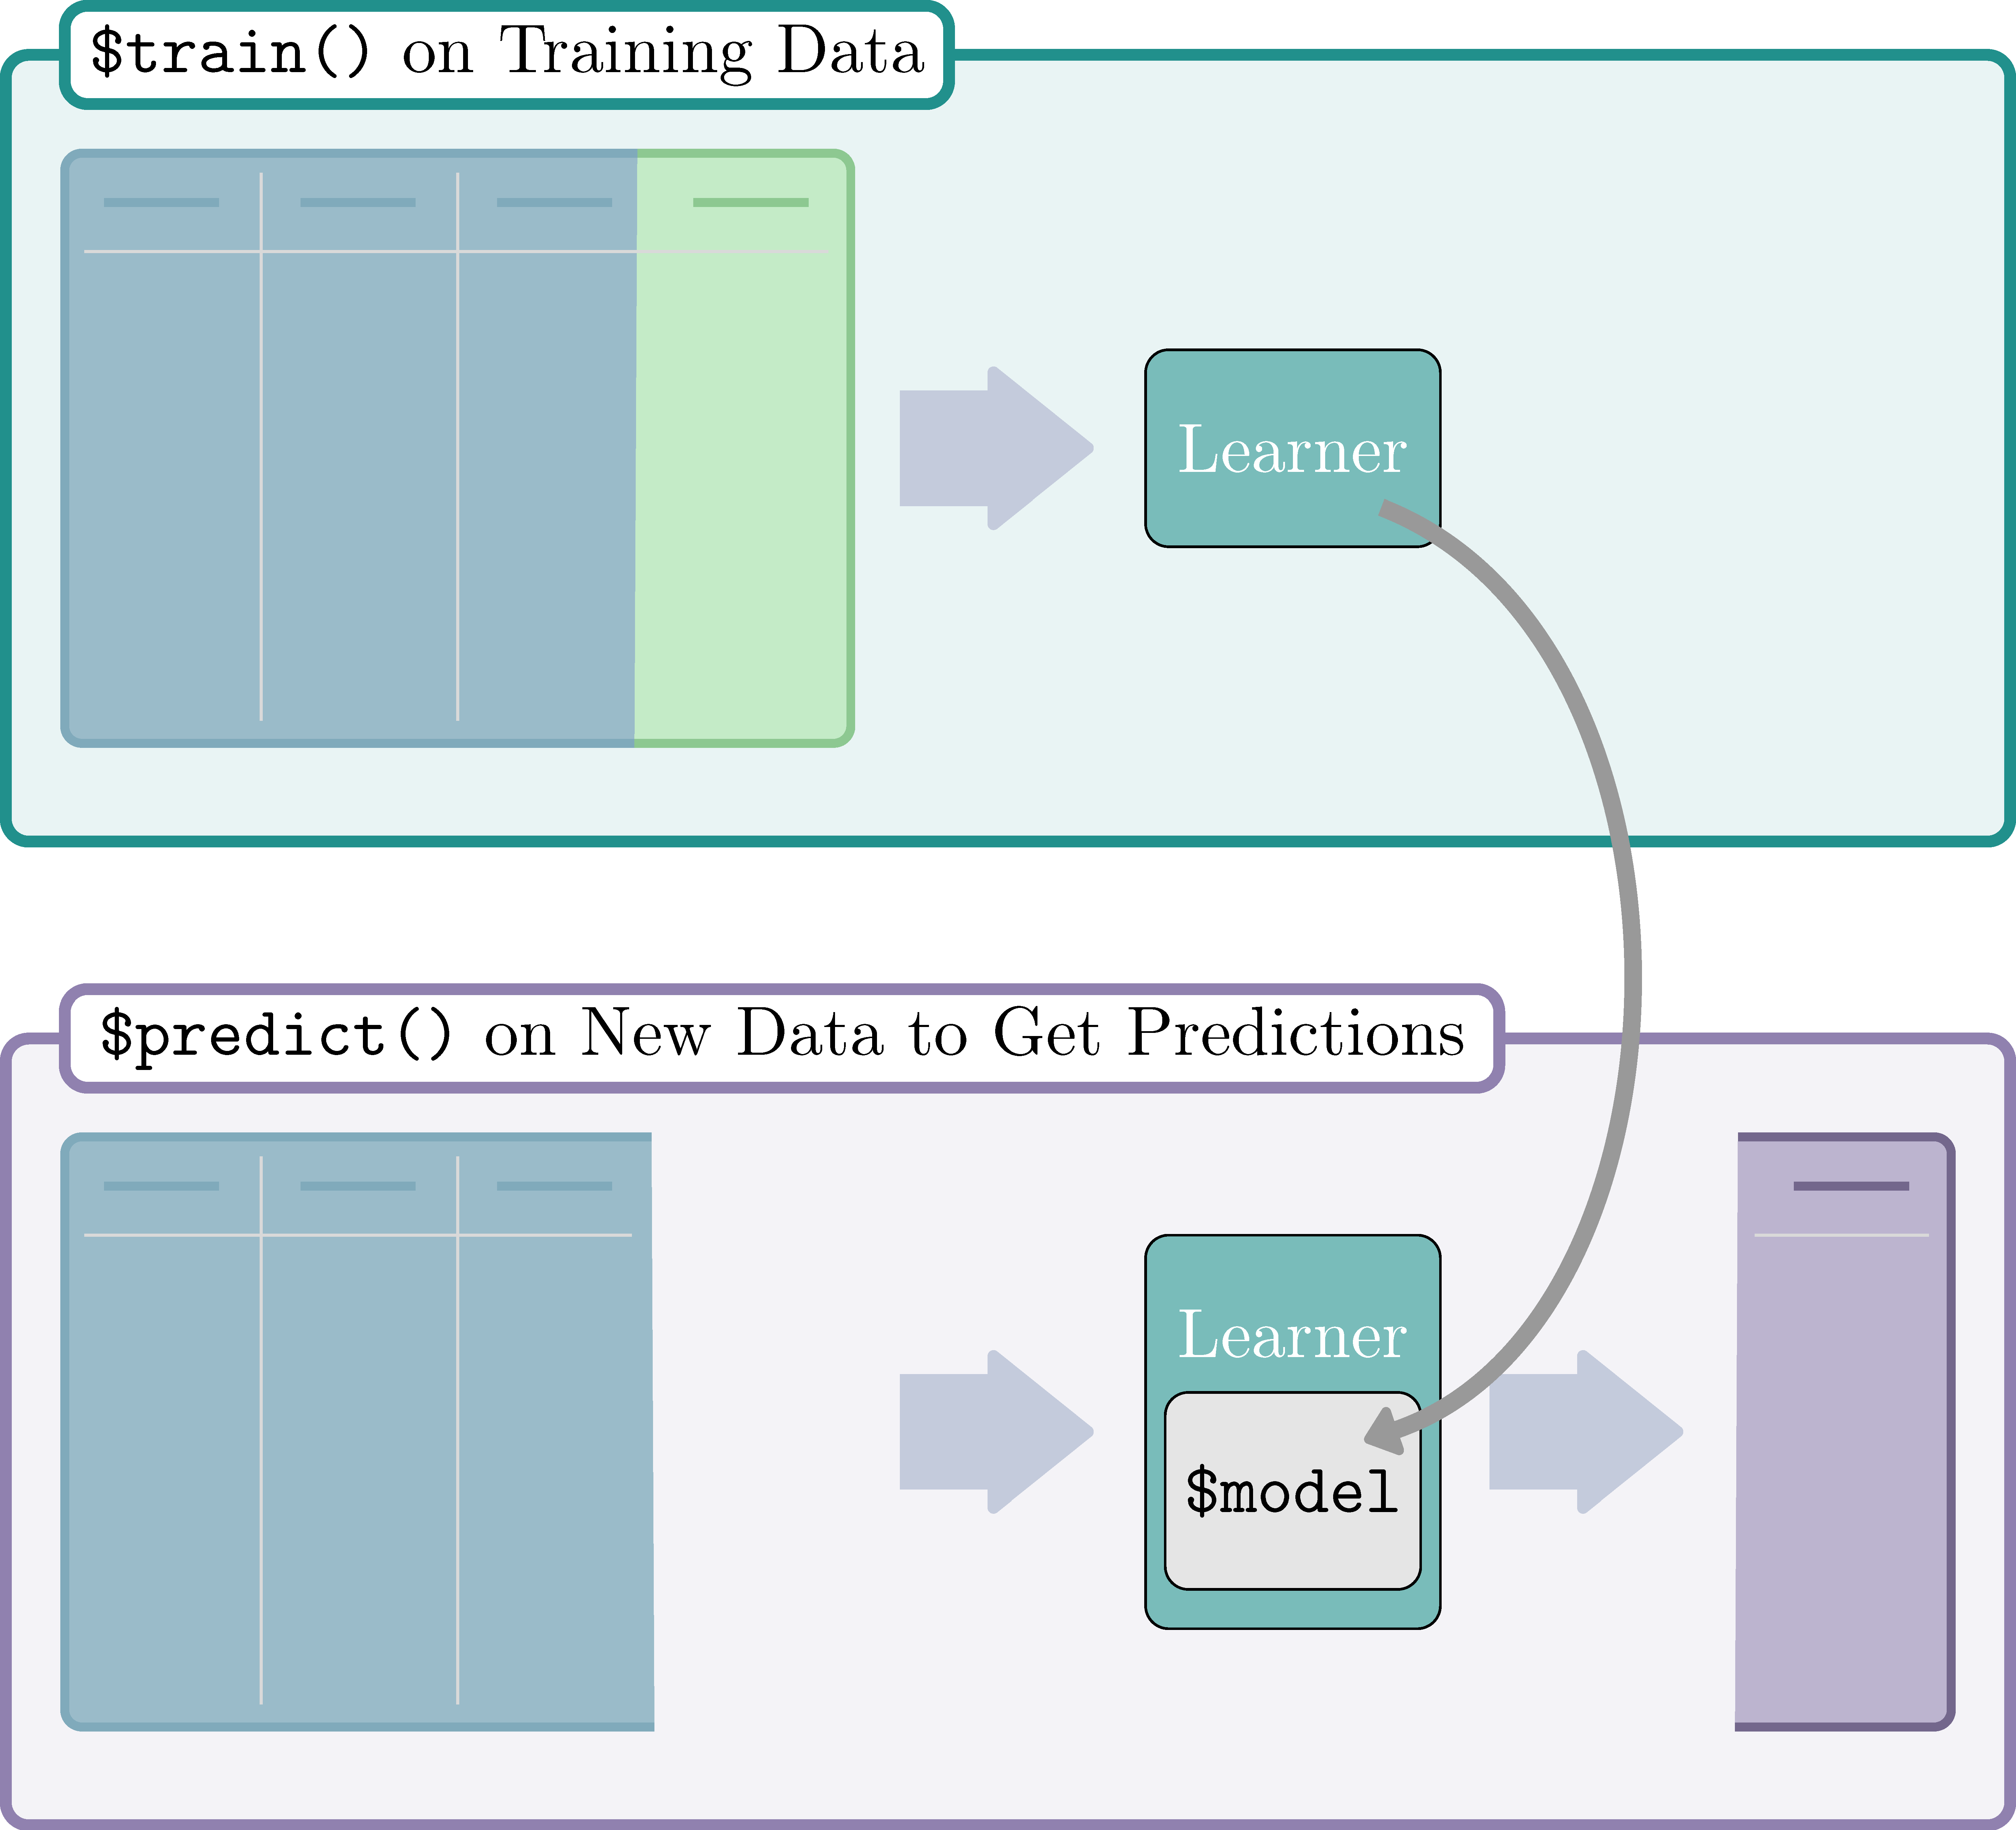
\includegraphics[width=0.7\textwidth,height=\textheight]{chapters/chapter2/Figures/mlr3book_figures-2.png}

}

\caption{\label{fig-basics-learner}Overview of the different stages of a
learner. Top -- data (features and a target) are passed to an
(untrained) learner. Bottom -- new data are passed to the trained model
which makes predictions for the `missing' target column.}

\end{figure}

\hypertarget{sec-training}{%
\subsection{Training}\label{sec-training}}

In the simplest use case, models are trained by passing a task to a
learner with the
\texttt{\$train()}\index{\texttt{Learner}!\texttt{\$train()}}{\marginnote{\begin{footnotesize}\$train()\end{footnotesize}}}
method:

\begin{Shaded}
\begin{Highlighting}[]
\CommentTok{\# load mtcars task}
\NormalTok{tsk\_mtcars }\OtherTok{=} \FunctionTok{tsk}\NormalTok{(}\StringTok{"mtcars"}\NormalTok{)}
\CommentTok{\# load a regression tree}
\NormalTok{lrn\_rpart }\OtherTok{=} \FunctionTok{lrn}\NormalTok{(}\StringTok{"regr.rpart"}\NormalTok{)}
\CommentTok{\# pass the task to the learner via $train()}
\NormalTok{lrn\_rpart}\SpecialCharTok{$}\FunctionTok{train}\NormalTok{(tsk\_mtcars)}
\end{Highlighting}
\end{Shaded}

After training, the fitted model is stored in the
\texttt{\$model}\index{\texttt{Learner}!\texttt{\$model}}{\marginnote{\begin{footnotesize}\$model\end{footnotesize}}}
field for future inspection and prediction:

\begin{Shaded}
\begin{Highlighting}[]
\CommentTok{\# inspect the trained model}
\NormalTok{lrn\_rpart}\SpecialCharTok{$}\NormalTok{model}
\end{Highlighting}
\end{Shaded}

\begin{verbatim}
n= 32 

node), split, n, deviance, yval
      * denotes terminal node

1) root 32 1126.00 20.09  
  2) cyl>=5 21  198.50 16.65  
    4) hp>=192.5 7   28.83 13.41 *
    5) hp< 192.5 14   59.87 18.26 *
  3) cyl< 5 11  203.40 26.66 *
\end{verbatim}

We see that the regression tree has identified features in the task that
are predictive of the target (\texttt{mpg}) and used them to partition
observations. The textual representation of the model depends on the
type of learner. For more information on any model see the learner help
page, which can be accessed in the same way as tasks with the
\texttt{help()} field, e.g., \texttt{lrn\_rpart\$help()}.

\hypertarget{sec-basics-partition}{%
\subsubsection{Partitioning Data}\label{sec-basics-partition}}

When assessing the quality of a model's predictions, you will likely
want to partition your dataset to get a fair and unbiased estimate of a
model's generalization error. In Chapter~\ref{sec-performance} we will
look at resampling and benchmark experiments, which will go into more
detail about performance estimation but for now, we will just discuss
the simplest method of splitting data using the
\href{https://mlr3.mlr-org.com/reference/partition.html}{\texttt{partition()}}\index{\texttt{partition()}}{\marginnote{\begin{footnotesize}\texttt{partition()}\end{footnotesize}}}
function. This function creates index sets that randomly split the given
task into two disjoint sets: a training set\index{training data} (67\%
of the total data by default) and a test set\index{test data} (the
remaining 33\% of the total data not in the training set).

\begin{Shaded}
\begin{Highlighting}[]
\NormalTok{splits }\OtherTok{=} \FunctionTok{partition}\NormalTok{(tsk\_mtcars)}
\NormalTok{splits}
\end{Highlighting}
\end{Shaded}

\begin{verbatim}
$train
 [1]  1  3  4  5  8 10 21 25 32  6  7 11 14 15 16 17 22 31 19 20 26

$test
 [1]  2  9 27 30 12 13 23 24 29 18 28
\end{verbatim}

When training we will tell the model to only use the training data by
passing the row IDs from \texttt{partition} to the \texttt{row\_ids}
argument of \texttt{\$train()}:

\begin{Shaded}
\begin{Highlighting}[]
\NormalTok{lrn\_rpart}\SpecialCharTok{$}\FunctionTok{train}\NormalTok{(tsk\_mtcars, }\AttributeTok{row\_ids =}\NormalTok{ splits}\SpecialCharTok{$}\NormalTok{train)}
\end{Highlighting}
\end{Shaded}

Now we can use our trained learner to make predictions on new data.

\hypertarget{sec-predicting}{%
\subsection{Predicting}\label{sec-predicting}}

Predicting from trained models is as simple as passing your data as a
\texttt{Task} to the
\texttt{\$predict()}\index{\texttt{Learner}!\texttt{\$predict()}}{\marginnote{\begin{footnotesize}\$predict()\end{footnotesize}}}
method of the trained \texttt{Learner}.

Carrying straight on from our last example, we will call the
\texttt{\$predict()} method of our trained learner and again will use
the \texttt{row\_ids} argument, but this time to pass the IDs of our
test set\index{test data}:

\begin{Shaded}
\begin{Highlighting}[]
\NormalTok{prediction }\OtherTok{=}\NormalTok{ lrn\_rpart}\SpecialCharTok{$}\FunctionTok{predict}\NormalTok{(tsk\_mtcars, }\AttributeTok{row\_ids =}\NormalTok{ splits}\SpecialCharTok{$}\NormalTok{test)}
\end{Highlighting}
\end{Shaded}

The \texttt{\$predict()} method returns an object inheriting from
\href{https://mlr3.mlr-org.com/reference/Prediction.html}{\texttt{Prediction}}\index{\texttt{Prediction}}{\marginnote{\begin{footnotesize}\texttt{Prediction}\end{footnotesize}}},
in this case
\href{https://mlr3.mlr-org.com/reference/PredictionRegr.html}{\texttt{PredictionRegr}}\index{\texttt{PredictionRegr}}{\marginnote{\begin{footnotesize}\texttt{PredictionRegr}\end{footnotesize}}}
as this is a regression task.

\begin{Shaded}
\begin{Highlighting}[]
\NormalTok{prediction}
\end{Highlighting}
\end{Shaded}

\begin{verbatim}
<PredictionRegr> for 11 observations:
    row_ids truth response
          2  21.0     24.9
          9  22.8     24.9
         27  26.0     24.9
---                       
         29  15.8     24.9
         18  32.4     24.9
         28  30.4     24.9
\end{verbatim}

The \texttt{row\_ids} column corresponds to the row IDs of the predicted
observations. The \texttt{truth} column contains the ground truth data
if available, which the object extracts from the task, in this case:
\texttt{tsk\_mtcars\$truth(splits\$test)}. Finally, the
\texttt{response} column contains the values predicted by the model. The
\texttt{Prediction} object can easily be converted into a
\texttt{data.table} or \texttt{data.frame} using
\texttt{as.data.table()}/\texttt{as.data.frame()} respectively.

All data in the above columns can be accessed directly, for example, to
get the first two predicted responses:

\begin{Shaded}
\begin{Highlighting}[]
\NormalTok{prediction}\SpecialCharTok{$}\NormalTok{response[}\DecValTok{1}\SpecialCharTok{:}\DecValTok{2}\NormalTok{]}
\end{Highlighting}
\end{Shaded}

\begin{verbatim}
[1] 24.9 24.9
\end{verbatim}

Similarly to plotting \texttt{Task}s,
\href{https://mlr3viz.mlr-org.com}{\texttt{mlr3viz}}\index{\texttt{mlr3viz}}
provides an
\href{https://www.rdocumentation.org/packages/ggplot2/topics/autoplot}{\texttt{autoplot()}}
method for \texttt{Prediction} objects.

\begin{Shaded}
\begin{Highlighting}[]
\FunctionTok{library}\NormalTok{(mlr3viz)}
\NormalTok{prediction }\OtherTok{=}\NormalTok{ lrn\_rpart}\SpecialCharTok{$}\FunctionTok{predict}\NormalTok{(tsk\_mtcars, splits}\SpecialCharTok{$}\NormalTok{test)}
\FunctionTok{autoplot}\NormalTok{(prediction)}
\end{Highlighting}
\end{Shaded}

\begin{figure}[H]

{\centering 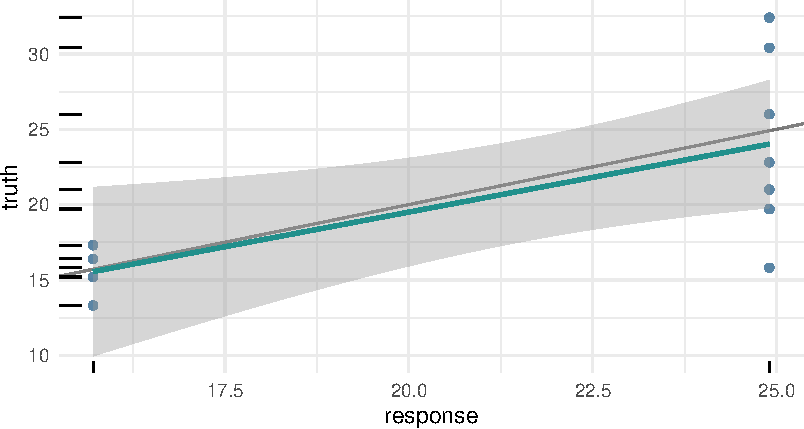
\includegraphics[width=0.7\textwidth,height=\textheight]{chapters/chapter2/data_and_basic_modeling_files/figure-pdf/fig-basics-truthresponse-1.pdf}

}

\caption{\label{fig-basics-truthresponse}Comparing predicted and ground
truth values for the mtcars dataset.}

\end{figure}

In the examples above we made predictions by passing a task to
\texttt{\$predict()}. However, if you would rather pass a
\texttt{data.frame} type object directly, then you can use
\texttt{\$predict\_newdata()}\index{\texttt{Learner}!\texttt{\$predict\_newdata()}}.
Note, the \texttt{truth} column values are all \texttt{NA}, as we did
not include a target column in the generated data.

\begin{Shaded}
\begin{Highlighting}[]
\NormalTok{mtcars\_new }\OtherTok{=} \FunctionTok{data.table}\NormalTok{(}\AttributeTok{cyl =} \FunctionTok{c}\NormalTok{(}\DecValTok{5}\NormalTok{, }\DecValTok{6}\NormalTok{), }\AttributeTok{disp =} \FunctionTok{c}\NormalTok{(}\DecValTok{100}\NormalTok{, }\DecValTok{120}\NormalTok{),}
  \AttributeTok{hp =} \FunctionTok{c}\NormalTok{(}\DecValTok{100}\NormalTok{, }\DecValTok{150}\NormalTok{), }\AttributeTok{drat =} \FunctionTok{c}\NormalTok{(}\DecValTok{4}\NormalTok{, }\FloatTok{3.9}\NormalTok{), }\AttributeTok{wt =} \FunctionTok{c}\NormalTok{(}\FloatTok{3.8}\NormalTok{, }\FloatTok{4.1}\NormalTok{),}
  \AttributeTok{qsec =} \FunctionTok{c}\NormalTok{(}\DecValTok{18}\NormalTok{, }\FloatTok{19.5}\NormalTok{), }\AttributeTok{vs =} \FunctionTok{c}\NormalTok{(}\DecValTok{1}\NormalTok{, }\DecValTok{0}\NormalTok{), }\AttributeTok{am =} \FunctionTok{c}\NormalTok{(}\DecValTok{1}\NormalTok{, }\DecValTok{1}\NormalTok{),}
  \AttributeTok{gear =} \FunctionTok{c}\NormalTok{(}\DecValTok{6}\NormalTok{, }\DecValTok{4}\NormalTok{), }\AttributeTok{carb =} \FunctionTok{c}\NormalTok{(}\DecValTok{3}\NormalTok{, }\DecValTok{5}\NormalTok{))}
\NormalTok{prediction }\OtherTok{=}\NormalTok{ lrn\_rpart}\SpecialCharTok{$}\FunctionTok{predict\_newdata}\NormalTok{(mtcars\_new)}
\NormalTok{prediction}
\end{Highlighting}
\end{Shaded}

\begin{verbatim}
<PredictionRegr> for 2 observations:
 row_ids truth response
       1    NA    15.71
       2    NA    15.71
\end{verbatim}

\hypertarget{changing-the-prediction-type}{%
\subsubsection*{Changing the Prediction
Type}\label{changing-the-prediction-type}}

While predicting a single numeric quantity is the most common prediction
type in regression, it is not the only prediction type. Several
regression models can also predict standard errors. To predict this, the
\texttt{\$predict\_type}\index{\texttt{Learner}!\texttt{\$predict\_type}}
field of a
\href{https://mlr3.mlr-org.com/reference/LearnerRegr.html}{\texttt{LearnerRegr}}
must be changed from ``response'' (the default) to \texttt{"se"} before
training. The \texttt{"rpart"} learner we used above does not support
predicting standard errors, so in the example below we will use a linear
regression model (\texttt{lrn("regr.lm")}).

\begin{Shaded}
\begin{Highlighting}[]
\FunctionTok{library}\NormalTok{(mlr3learners)}
\NormalTok{lrn\_lm }\OtherTok{=} \FunctionTok{lrn}\NormalTok{(}\StringTok{"regr.lm"}\NormalTok{, }\AttributeTok{predict\_type =} \StringTok{"se"}\NormalTok{)}
\NormalTok{lrn\_lm}\SpecialCharTok{$}\FunctionTok{train}\NormalTok{(tsk\_mtcars, splits}\SpecialCharTok{$}\NormalTok{train)}
\NormalTok{lrn\_lm}\SpecialCharTok{$}\FunctionTok{predict}\NormalTok{(tsk\_mtcars, splits}\SpecialCharTok{$}\NormalTok{test)}
\end{Highlighting}
\end{Shaded}

\begin{verbatim}
<PredictionRegr> for 11 observations:
    row_ids truth response    se
          2  21.0    20.20 1.817
          9  22.8    33.32 4.246
         27  26.0    32.22 4.121
---                             
         29  15.8    28.26 4.182
         18  32.4    27.77 1.114
         28  30.4    27.57 2.735
\end{verbatim}

Now the output includes an \texttt{se} column as desired. In
Section~\ref{sec-basics-classif-learner} we will see prediction types
playing an even bigger role in the context of classification.

Having covered the unified train/predict interface, we can now look at
how to use hyperparameters to configure these methods for individual
algorithms.

\hypertarget{sec-param-set}{%
\subsection{Hyperparameters}\label{sec-param-set}}

\texttt{Learner}s encapsulate a machine learning algorithm and its
hyperparameters\index{hyperparameters}, which affect \emph{how} the
algorithm is run and can be set by the user. Hyperparameters may affect
how a model is trained or how it makes predictions and deciding how to
set hyperparameters can require expert knowledge. Hyperparameters can be
optimized automatically (Chapter~\ref{sec-optimization}), but in this
chapter we will focus on how to set them manually.

\hypertarget{paradox-and-parameter-sets}{%
\subsubsection{Paradox and Parameter
Sets}\label{paradox-and-parameter-sets}}

We will continue our running example with a regression tree learner. To
access the hyperparameters in the decision tree, we use
\texttt{\$param\_set}\index{\texttt{Learner}!\texttt{\$param\_set}}{\marginnote{\begin{footnotesize}\$param\_set\end{footnotesize}}}:

\begin{Shaded}
\begin{Highlighting}[]
\NormalTok{lrn\_rpart}\SpecialCharTok{$}\NormalTok{param\_set}
\end{Highlighting}
\end{Shaded}

\begin{verbatim}
<ParamSet>
                id    class lower upper nlevels        default value
 1:             cp ParamDbl     0     1     Inf           0.01      
 2:     keep_model ParamLgl    NA    NA       2          FALSE      
 3:     maxcompete ParamInt     0   Inf     Inf              4      
 4:       maxdepth ParamInt     1    30      30             30      
 5:   maxsurrogate ParamInt     0   Inf     Inf              5      
 6:      minbucket ParamInt     1   Inf     Inf <NoDefault[3]>      
 7:       minsplit ParamInt     1   Inf     Inf             20      
 8: surrogatestyle ParamInt     0     1       2              0      
 9:   usesurrogate ParamInt     0     2       3              2      
10:           xval ParamInt     0   Inf     Inf             10     0
\end{verbatim}

The output above is a
\href{https://paradox.mlr-org.com/reference/ParamSet.html}{\texttt{ParamSet}}\index{\texttt{ParamSet}}{\marginnote{\begin{footnotesize}\texttt{ParamSet}\end{footnotesize}}}
object, supplied by the
\href{https://paradox.mlr-org.com}{\texttt{paradox}} package. These
objects provide information on hyperparameters including their name
(\texttt{id}), data type (\texttt{class}), technically valid ranges for
hyperparameter values (\texttt{lower}, \texttt{upper}), the number of
levels possible if the data type is categorical (\texttt{nlevels}), the
default value from the underlying package (\texttt{default}), and
finally the set value (\texttt{value}). The second column references
classes defined in \href{https://paradox.mlr-org.com}{\texttt{paradox}}
that determine the class of the parameter and the possible values it can
take. Table~\ref{tbl-parameters-classes} lists the possible
hyperparameter types, all of which inherit from
\href{https://paradox.mlr-org.com/reference/Param.html}{\texttt{Param}}.

\hypertarget{tbl-parameters-classes}{}
\begin{longtable}[]{@{}
  >{\raggedright\arraybackslash}p{(\columnwidth - 2\tabcolsep) * \real{0.3333}}
  >{\raggedright\arraybackslash}p{(\columnwidth - 2\tabcolsep) * \real{0.6667}}@{}}
\caption{\label{tbl-parameters-classes}Hyperparameter classes and the
type of hyperparameter they represent.}\tabularnewline
\toprule\noalign{}
\begin{minipage}[b]{\linewidth}\raggedright
Hyperparameter Class
\end{minipage} & \begin{minipage}[b]{\linewidth}\raggedright
Hyperparameter Type
\end{minipage} \\
\midrule\noalign{}
\endfirsthead
\toprule\noalign{}
\begin{minipage}[b]{\linewidth}\raggedright
Hyperparameter Class
\end{minipage} & \begin{minipage}[b]{\linewidth}\raggedright
Hyperparameter Type
\end{minipage} \\
\midrule\noalign{}
\endhead
\bottomrule\noalign{}
\endlastfoot
\href{https://paradox.mlr-org.com/reference/ParamDbl.html}{\texttt{ParamDbl}}\index{\texttt{ParamDbl}}
& Real-valued (numeric) \\
\href{https://paradox.mlr-org.com/reference/ParamInt.html}{\texttt{ParamInt}}\index{\texttt{ParamInt}}
& Integer \\
\href{https://paradox.mlr-org.com/reference/ParamFct.html}{\texttt{ParamFct}}\index{\texttt{ParamFct}}
& Categorical (factor) \\
\href{https://paradox.mlr-org.com/reference/ParamLgl.html}{\texttt{ParamLgl}}\index{\texttt{ParamLgl}}
& Logical / Boolean \\
\href{https://paradox.mlr-org.com/reference/ParamUty.html}{\texttt{ParamUty}}\index{\texttt{ParamUty}}
& Untyped \\
\end{longtable}

In our decision tree example, we can infer from the \texttt{ParamSet}
output that:

\begin{itemize}
\tightlist
\item
  \texttt{cp} must be a ``double'' (\texttt{ParamDbl}) taking values
  between \texttt{0} (\texttt{lower}) and \texttt{1} (\texttt{upper})
  with a default of 0.01 (\texttt{default}).
\item
  \texttt{keep\_model} must be a ``logical'' (\texttt{ParamLgl}) taking
  values \texttt{TRUE} or \texttt{FALSE} with default \texttt{FALSE}
\item
  \texttt{xval} must be an ``integer'' (\texttt{ParamInt}) taking values
  between \texttt{0} and \texttt{Inf} with a default of \texttt{10} and
  has a set value of \texttt{0}.
\end{itemize}

In rare cases (we try to minimize it as much as possible),
hyperparameters are initialized to values which deviate from the default
in the underlying package. When this happens, the reason will always be
given in the learner help page. In the case of
\texttt{lrn("regr.rpart")}, the \texttt{xval} hyperparameter is
initialized to \texttt{0} because \texttt{xval} controls internal
cross-validations and if a user accidentally leaves this at the default
\texttt{10}, model training can take an unnecessarily long time.

\hypertarget{getting-and-setting-hyperparameter-values}{%
\subsubsection{Getting and Setting Hyperparameter
Values}\label{getting-and-setting-hyperparameter-values}}

Now we have looked at how hyperparameter sets are stored, we can think
about getting and setting them. Returning to our decision tree, say we
are interested in growing a tree with depth \texttt{1}, also known as a
``decision stump'', where data is split only once into two terminal
nodes. From the parameter set output, we know that the \texttt{maxdepth}
parameter has a default of \texttt{30} and that it takes integer values.

There are a few different ways we could change this hyperparameter. The
simplest way is during construction of the learner by passing the
hyperparameter name and new value to \texttt{lrn()}:

\begin{Shaded}
\begin{Highlighting}[]
\NormalTok{lrn\_rpart }\OtherTok{=} \FunctionTok{lrn}\NormalTok{(}\StringTok{"regr.rpart"}\NormalTok{, }\AttributeTok{maxdepth =} \DecValTok{1}\NormalTok{)}
\end{Highlighting}
\end{Shaded}

We can get a list of non-default hyperparameters (i.e., those that have
been set) by using \texttt{\$param\_set\$values}:

\begin{Shaded}
\begin{Highlighting}[]
\NormalTok{lrn\_rpart}\SpecialCharTok{$}\NormalTok{param\_set}\SpecialCharTok{$}\NormalTok{values}
\end{Highlighting}
\end{Shaded}

\begin{verbatim}
$xval
[1] 0

$maxdepth
[1] 1
\end{verbatim}

Now we can see that \texttt{maxdepth\ =\ 1} (as we discussed above
\texttt{xval\ =\ 0} is changed during construction) and the learned
regression tree reflects this:

\begin{Shaded}
\begin{Highlighting}[]
\NormalTok{lrn\_rpart}\SpecialCharTok{$}\FunctionTok{train}\NormalTok{(}\FunctionTok{tsk}\NormalTok{(}\StringTok{"mtcars"}\NormalTok{))}\SpecialCharTok{$}\NormalTok{model}
\end{Highlighting}
\end{Shaded}

\begin{verbatim}
n= 32 

node), split, n, deviance, yval
      * denotes terminal node

1) root 32 1126.0 20.09  
  2) cyl>=5 21  198.5 16.65 *
  3) cyl< 5 11  203.4 26.66 *
\end{verbatim}

The \texttt{\$values} field simply returns a \texttt{list} of set
hyperparameters, so another way to update hyperparameters is by updating
an element in the list:

\begin{Shaded}
\begin{Highlighting}[]
\NormalTok{lrn\_rpart}\SpecialCharTok{$}\NormalTok{param\_set}\SpecialCharTok{$}\NormalTok{values}\SpecialCharTok{$}\NormalTok{maxdepth }\OtherTok{=} \DecValTok{2}
\NormalTok{lrn\_rpart}\SpecialCharTok{$}\NormalTok{param\_set}\SpecialCharTok{$}\NormalTok{values}
\end{Highlighting}
\end{Shaded}

\begin{verbatim}
$xval
[1] 0

$maxdepth
[1] 2
\end{verbatim}

\begin{Shaded}
\begin{Highlighting}[]
\CommentTok{\# now with depth 2}
\NormalTok{lrn\_rpart}\SpecialCharTok{$}\FunctionTok{train}\NormalTok{(}\FunctionTok{tsk}\NormalTok{(}\StringTok{"mtcars"}\NormalTok{))}\SpecialCharTok{$}\NormalTok{model}
\end{Highlighting}
\end{Shaded}

\begin{verbatim}
n= 32 

node), split, n, deviance, yval
      * denotes terminal node

1) root 32 1126.00 20.09  
  2) cyl>=5 21  198.50 16.65  
    4) hp>=192.5 7   28.83 13.41 *
    5) hp< 192.5 14   59.87 18.26 *
  3) cyl< 5 11  203.40 26.66 *
\end{verbatim}

To set multiple values at once we recommend either setting these during
construction or using
\texttt{\$set\_values()}\index{\texttt{Learner}!\texttt{\$set\_values()}}{\marginnote{\begin{footnotesize}\$set\_values()\end{footnotesize}}},
which updates the given hyperparameters (argument names) with the
respective values.

\begin{Shaded}
\begin{Highlighting}[]
\NormalTok{lrn\_rpart }\OtherTok{=} \FunctionTok{lrn}\NormalTok{(}\StringTok{"regr.rpart"}\NormalTok{, }\AttributeTok{maxdepth =} \DecValTok{3}\NormalTok{, }\AttributeTok{xval =} \DecValTok{1}\NormalTok{)}
\NormalTok{lrn\_rpart}\SpecialCharTok{$}\NormalTok{param\_set}\SpecialCharTok{$}\NormalTok{values}
\end{Highlighting}
\end{Shaded}

\begin{verbatim}
$xval
[1] 1

$maxdepth
[1] 3
\end{verbatim}

\begin{Shaded}
\begin{Highlighting}[]
\CommentTok{\# or with set\_values}
\NormalTok{lrn\_rpart}\SpecialCharTok{$}\NormalTok{param\_set}\SpecialCharTok{$}\FunctionTok{set\_values}\NormalTok{(}\AttributeTok{xval =} \DecValTok{2}\NormalTok{, }\AttributeTok{cp =} \FloatTok{0.5}\NormalTok{)}
\NormalTok{lrn\_rpart}\SpecialCharTok{$}\NormalTok{param\_set}\SpecialCharTok{$}\NormalTok{values}
\end{Highlighting}
\end{Shaded}

\begin{verbatim}
$xval
[1] 2

$maxdepth
[1] 3

$cp
[1] 0.5
\end{verbatim}

\begin{tcolorbox}[enhanced jigsaw, opacitybacktitle=0.6, rightrule=.15mm, opacityback=0, arc=.35mm, breakable, titlerule=0mm, colframe=quarto-callout-warning-color-frame, coltitle=black, bottomrule=.15mm, toprule=.15mm, colback=white, colbacktitle=quarto-callout-warning-color!10!white, bottomtitle=1mm, toptitle=1mm, title=\textcolor{quarto-callout-warning-color}{\faExclamationTriangle}\hspace{0.5em}{Setting Hyperparameters Using a \texttt{list}}, leftrule=.75mm, left=2mm]

As \texttt{lrn\_rpart\$param\_set\$values} returns a \texttt{list}, some
users may be tempted to set hyperparameters by passing a new
\texttt{list} to \texttt{\$values} -- this would work but \textbf{we do
not recommend it}. This is because passing a \texttt{list} will wipe any
existing hyperparameter values if they are not included in the list. For
example:

\begin{Shaded}
\begin{Highlighting}[]
\CommentTok{\# set xval and cp}
\NormalTok{lrn\_rpart\_params }\OtherTok{=} \FunctionTok{lrn}\NormalTok{(}\StringTok{"regr.rpart"}\NormalTok{, }\AttributeTok{xval =} \DecValTok{0}\NormalTok{, }\AttributeTok{cp =} \DecValTok{1}\NormalTok{)}
\CommentTok{\# passing maxdepth through a list, removing all other values}
\NormalTok{lrn\_rpart\_params}\SpecialCharTok{$}\NormalTok{param\_set}\SpecialCharTok{$}\NormalTok{values }\OtherTok{=} \FunctionTok{list}\NormalTok{(}\AttributeTok{maxdepth =} \DecValTok{1}\NormalTok{)}
\CommentTok{\# we have removed xval and cp by mistake}
\NormalTok{lrn\_rpart\_params}\SpecialCharTok{$}\NormalTok{param\_set}\SpecialCharTok{$}\NormalTok{values}
\end{Highlighting}
\end{Shaded}

\begin{verbatim}
$maxdepth
[1] 1
\end{verbatim}

\begin{Shaded}
\begin{Highlighting}[]
\CommentTok{\# now with set\_values}
\NormalTok{lrn\_rpart\_params }\OtherTok{=} \FunctionTok{lrn}\NormalTok{(}\StringTok{"regr.rpart"}\NormalTok{, }\AttributeTok{xval =} \DecValTok{0}\NormalTok{, }\AttributeTok{cp =} \DecValTok{1}\NormalTok{)}
\NormalTok{lrn\_rpart\_params}\SpecialCharTok{$}\NormalTok{param\_set}\SpecialCharTok{$}\FunctionTok{set\_values}\NormalTok{(}\AttributeTok{maxdepth =} \DecValTok{1}\NormalTok{)}
\NormalTok{lrn\_rpart\_params}\SpecialCharTok{$}\NormalTok{param\_set}\SpecialCharTok{$}\NormalTok{values}
\end{Highlighting}
\end{Shaded}

\begin{verbatim}
$xval
[1] 0

$cp
[1] 1

$maxdepth
[1] 1
\end{verbatim}

\end{tcolorbox}

Whichever method you choose, all have safety checks to ensure your new
values fall within the allowed parameter range:

\begin{Shaded}
\begin{Highlighting}[]
\FunctionTok{lrn}\NormalTok{(}\StringTok{"regr.rpart"}\NormalTok{, }\AttributeTok{cp =} \DecValTok{2}\NormalTok{, }\AttributeTok{maxdepth =} \DecValTok{2}\NormalTok{)}
\end{Highlighting}
\end{Shaded}

\begin{verbatim}
Error in self$assert(xs): Assertion on 'xs' failed: cp:
	Element 1 is not <= 1.
\end{verbatim}

\hypertarget{hyperparameter-dependencies}{%
\subsubsection{Hyperparameter
Dependencies}\label{hyperparameter-dependencies}}

\begin{tcolorbox}[enhanced jigsaw, colframe=quarto-callout-note-color-frame, rightrule=.15mm, bottomrule=.15mm, toprule=.15mm, opacityback=0, colback=white, left=2mm, arc=.35mm, breakable, leftrule=.75mm]
\begin{minipage}[t]{5.5mm}
\textcolor{quarto-callout-note-color}{\faInfo}
\end{minipage}%
\begin{minipage}[t]{\textwidth - 5.5mm}

\textbf{This section covers advanced ML or technical
details.}\vspace{2mm}

\end{minipage}%
\end{tcolorbox}

More complex hyperparameter spaces may include dependencies, which occur
when setting a hyperparameter is conditional on the value of another
hyperparameter; this is most important in the context of model tuning
(Chapter~\ref{sec-optimization}). One such example is a support vector
machine\index{support vector machine} (\texttt{lrn("regr.svm")}). The
field \texttt{\$deps}\index{\texttt{ParamSet}!\texttt{\$deps}} returns a
\texttt{data.table}, which lists the hyperparameter dependencies in the
\texttt{Learner}. For example we can see that the \texttt{cost}
(\texttt{id}-column) parameter is dependent on the \texttt{type}
(\texttt{on}-column) parameter.

\begin{Shaded}
\begin{Highlighting}[]
\FunctionTok{lrn}\NormalTok{(}\StringTok{"regr.svm"}\NormalTok{)}\SpecialCharTok{$}\NormalTok{param\_set}\SpecialCharTok{$}\NormalTok{deps}
\end{Highlighting}
\end{Shaded}

\begin{verbatim}
        id     on           cond
1:    cost   type <CondAnyOf[9]>
2:      nu   type <CondEqual[9]>
3:  degree kernel <CondEqual[9]>
4:   coef0 kernel <CondAnyOf[9]>
5:   gamma kernel <CondAnyOf[9]>
6: epsilon   type <CondEqual[9]>
\end{verbatim}

The \texttt{cond} column tells us what the condition is, which will
either mean that \texttt{id} can be set if \texttt{on} equals a single
value
(\href{https://paradox.mlr-org.com/reference/Condition.html}{\texttt{CondEqual}})
or any value in the listed set
(\href{https://paradox.mlr-org.com/reference/Condition.html}{\texttt{CondAnyOf}}).

\begin{Shaded}
\begin{Highlighting}[]
\FunctionTok{lrn}\NormalTok{(}\StringTok{"regr.svm"}\NormalTok{)}\SpecialCharTok{$}\NormalTok{param\_set}\SpecialCharTok{$}\NormalTok{deps[[}\DecValTok{1}\NormalTok{, }\StringTok{"cond"}\NormalTok{]]}
\end{Highlighting}
\end{Shaded}

\begin{verbatim}
CondAnyOf: x ∈ {eps-regression, nu-regression}
\end{verbatim}

\begin{Shaded}
\begin{Highlighting}[]
\FunctionTok{lrn}\NormalTok{(}\StringTok{"regr.svm"}\NormalTok{)}\SpecialCharTok{$}\NormalTok{param\_set}\SpecialCharTok{$}\NormalTok{deps[[}\DecValTok{3}\NormalTok{, }\StringTok{"cond"}\NormalTok{]]}
\end{Highlighting}
\end{Shaded}

\begin{verbatim}
CondEqual: x = polynomial
\end{verbatim}

This tells us that the parameter \texttt{cost} should only be set if the
\texttt{type} parameter is one of \texttt{"eps-regression"} or
\texttt{"nu-regression"}, and \texttt{degree} should only be set if
\texttt{kernel} is equal to \texttt{"polynomial"}.

The \texttt{Learner} will error if dependent hyperparameters are set
when their conditions are not met:

\begin{Shaded}
\begin{Highlighting}[]
\CommentTok{\# error as kernel is not polynomial}
\FunctionTok{lrn}\NormalTok{(}\StringTok{"regr.svm"}\NormalTok{, }\AttributeTok{kernel =} \StringTok{"linear"}\NormalTok{, }\AttributeTok{degree =} \DecValTok{1}\NormalTok{)}
\end{Highlighting}
\end{Shaded}

\begin{verbatim}
Error in self$assert(xs): Assertion on 'xs' failed: The parameter 'degree'
	can only be set if the following condition is met 'kernel = polynomial'.
	Instead the current parameter value is: kernel=linear.
\end{verbatim}

\begin{Shaded}
\begin{Highlighting}[]
\CommentTok{\# works because kernel is polynomial}
\FunctionTok{lrn}\NormalTok{(}\StringTok{"regr.svm"}\NormalTok{, }\AttributeTok{kernel =} \StringTok{"polynomial"}\NormalTok{, }\AttributeTok{degree =} \DecValTok{1}\NormalTok{)}
\end{Highlighting}
\end{Shaded}

\begin{verbatim}
<LearnerRegrSVM:regr.svm>
* Model: -
* Parameters: kernel=polynomial, degree=1
* Packages: mlr3, mlr3learners, e1071
* Predict Types:  [response]
* Feature Types: logical, integer, numeric
* Properties: -
\end{verbatim}

\hypertarget{sec-basics-featureless}{%
\subsection{Baseline Learners}\label{sec-basics-featureless}}

Before we move on to learner evaluation, we will highlight an important
class of learners. These are extremely simple or `weak' learners known
as
baselines\index{baselines}{\marginnote{\begin{footnotesize}Baselines\end{footnotesize}}}.
Baselines are useful in model comparison (Chapter~\ref{sec-performance})
and as fallback learners (Section~\ref{sec-encapsulation-fallback},
Section~\ref{sec-fallback}). For regression, we have implemented the
baseline \texttt{lrn("regr.featureless")}, which always predicts new
values to be the mean (or median, if the \texttt{robust} hyperparameter
is set to \texttt{TRUE}) of the target in the training data:

\begin{Shaded}
\begin{Highlighting}[]
\CommentTok{\# generate data}
\NormalTok{df }\OtherTok{=} \FunctionTok{as\_task\_regr}\NormalTok{(}\FunctionTok{data.frame}\NormalTok{(}\AttributeTok{x =} \FunctionTok{runif}\NormalTok{(}\DecValTok{1000}\NormalTok{), }\AttributeTok{y =} \FunctionTok{rnorm}\NormalTok{(}\DecValTok{1000}\NormalTok{, }\DecValTok{2}\NormalTok{, }\DecValTok{1}\NormalTok{)),}
  \AttributeTok{target =} \StringTok{"y"}\NormalTok{)}
\FunctionTok{lrn}\NormalTok{(}\StringTok{"regr.featureless"}\NormalTok{)}\SpecialCharTok{$}\FunctionTok{train}\NormalTok{(df, }\DecValTok{1}\SpecialCharTok{:}\DecValTok{995}\NormalTok{)}\SpecialCharTok{$}\FunctionTok{predict}\NormalTok{(df, }\DecValTok{996}\SpecialCharTok{:}\DecValTok{1000}\NormalTok{)}
\end{Highlighting}
\end{Shaded}

\begin{verbatim}
<PredictionRegr> for 5 observations:
 row_ids truth response
     996 2.996    1.976
     997 3.675    1.976
     998 3.651    1.976
     999 1.803    1.976
    1000 1.196    1.976
\end{verbatim}

It is good practice to test all new models against a baseline, and also
to include baselines in experiments with multiple other models. In
general, a model that does not outperform a baseline is a `bad' model,
on the other hand, a model is not necessarily `good' if it outperforms
the baseline.

\hypertarget{sec-eval}{%
\section{Evaluation}\label{sec-eval}}

Perhaps \emph{the most} important step of the applied machine learning
workflow is evaluating model performance. Without this, we would have no
way to know if our trained model makes very accurate predictions, is
worse than randomly guessing, or somewhere in between. We will continue
with our decision tree example to establish if the quality of our
predictions is `good', first we will rerun the above code so it is
easier to follow along.

\begin{Shaded}
\begin{Highlighting}[]
\NormalTok{lrn\_rpart }\OtherTok{=} \FunctionTok{lrn}\NormalTok{(}\StringTok{"regr.rpart"}\NormalTok{)}
\NormalTok{tsk\_mtcars }\OtherTok{=} \FunctionTok{tsk}\NormalTok{(}\StringTok{"mtcars"}\NormalTok{)}
\NormalTok{splits }\OtherTok{=} \FunctionTok{partition}\NormalTok{(tsk\_mtcars)}
\NormalTok{lrn\_rpart}\SpecialCharTok{$}\FunctionTok{train}\NormalTok{(tsk\_mtcars, splits}\SpecialCharTok{$}\NormalTok{train)}
\NormalTok{prediction }\OtherTok{=}\NormalTok{ lrn\_rpart}\SpecialCharTok{$}\FunctionTok{predict}\NormalTok{(tsk\_mtcars, splits}\SpecialCharTok{$}\NormalTok{test)}
\end{Highlighting}
\end{Shaded}

\hypertarget{measures}{%
\subsection{Measures}\label{measures}}

The quality of predictions is evaluated using measures that compare them
to the ground truth data for supervised learning tasks. Similarly to
\texttt{Task}s and \texttt{Learner}s, the available measures in
\texttt{mlr3} are stored in a dictionary called
\href{https://mlr3.mlr-org.com/reference/mlr_measures.html}{\texttt{mlr\_measures}}\index{\texttt{mlr\_measures}}
and can be accessed with
\texttt{msr()}\index{\texttt{msr()/msrs()}}{\marginnote{\begin{footnotesize}msr()\end{footnotesize}}}:

\begin{Shaded}
\begin{Highlighting}[]
\FunctionTok{as.data.table}\NormalTok{(}\FunctionTok{msr}\NormalTok{())}
\end{Highlighting}
\end{Shaded}

\begin{verbatim}
             key                          label task_type
 1:          aic   Akaike Information Criterion      <NA>
 2:          bic Bayesian Information Criterion      <NA>
 3:  classif.acc        Classification Accuracy   classif
 4:  classif.auc       Area Under the ROC Curve   classif
 5: classif.bacc              Balanced Accuracy   classif
---                                                      
62:  sim.jaccard       Jaccard Similarity Index      <NA>
63:      sim.phi     Phi Coefficient Similarity      <NA>
64:    time_both                   Elapsed Time      <NA>
65: time_predict                   Elapsed Time      <NA>
66:   time_train                   Elapsed Time      <NA>
3 variables not shown: [packages, predict_type, task_properties]
\end{verbatim}

All measures implemented in \texttt{mlr3} are defined primarily by three
components: 1) the function that defines the measure; 2) whether a lower
or higher value is considered `good'; and 3) the range of possible
values the measure can take. As well as these defining elements, other
metadata are important to consider when selecting and using a
\texttt{Measure}, including if the measure has any special properties
(e.g., requires training data), the type of predictions the measure can
evaluate, and whether the measure has any `control parameters'. All this
information is encapsulated in the
\href{https://mlr3.mlr-org.com/reference/Measure.html}{\texttt{Measure}}\index{\texttt{Measure}}{\marginnote{\begin{footnotesize}\texttt{Measure}\end{footnotesize}}}
object. By example, let us consider the mean absolute
error\index{mean absolute error} (MAE):

\begin{Shaded}
\begin{Highlighting}[]
\NormalTok{measure }\OtherTok{=} \FunctionTok{msr}\NormalTok{(}\StringTok{"regr.mae"}\NormalTok{)}
\NormalTok{measure}
\end{Highlighting}
\end{Shaded}

\begin{verbatim}
<MeasureRegrSimple:regr.mae>: Mean Absolute Error
* Packages: mlr3, mlr3measures
* Range: [0, Inf]
* Minimize: TRUE
* Average: macro
* Parameters: list()
* Properties: -
* Predict type: response
\end{verbatim}

This measure compares the absolute difference (`error') between true and
predicted values: \(f(y, \hat{y}) = | y - \hat{y} |\). Lower values are
considered better (\texttt{Minimize:\ TRUE}), which is intuitive as we
would like the true values, \(y\), to be identical (or as close as
possible) in value to the predicted values, \(\hat{y}\). We can see that
the range of possible values the learner can take is from \(0\) to
\(\infty\) (\texttt{Range:\ {[}0,\ Inf{]}}), it has no special
properties (\texttt{Properties:\ -}), it evaluates \texttt{response}
type predictions for regression models
(\texttt{Predict\ type:\ response}), and it has no control parameters
(\texttt{Parameters:\ list()}).

Now let us see how to use this measure for scoring our predictions.

\hypertarget{scoring-predictions}{%
\subsection{Scoring Predictions}\label{scoring-predictions}}

Usually, supervised learning measures compare the difference between
predicted values and the ground truth. \texttt{mlr3} simplifies the
process of bringing these quantities together by storing the predictions
and true outcomes in the
\href{https://mlr3.mlr-org.com/reference/Prediction.html}{\texttt{Prediction}}\index{\texttt{Prediction}}
object as we have already seen.

\begin{Shaded}
\begin{Highlighting}[]
\NormalTok{prediction}
\end{Highlighting}
\end{Shaded}

\begin{verbatim}
<PredictionRegr> for 11 observations:
    row_ids truth response
          2  21.0    16.70
          8  24.4    26.81
         21  21.5    26.81
---                       
         31  15.0    16.70
         18  32.4    26.81
         26  27.3    26.81
\end{verbatim}

To calculate model performance, we simply call the
\texttt{\$score()}\index{\texttt{Prediction}!\texttt{\$score()}}{\marginnote{\begin{footnotesize}\$score()\end{footnotesize}}}
method of a \texttt{Prediction} object and pass as a single argument the
measure that we want to compute:

\begin{Shaded}
\begin{Highlighting}[]
\NormalTok{prediction}\SpecialCharTok{$}\FunctionTok{score}\NormalTok{(measure)}
\end{Highlighting}
\end{Shaded}

\begin{verbatim}
regr.mae 
   2.591 
\end{verbatim}

Note that all task types have default measures that are used if the
argument to \texttt{\$score()} is omitted, for regression this is the
mean squared error (\texttt{msr("regr.mse")}), which is the squared
difference between true and predicted values:
\(f(y, \hat{y}) = (y - \hat{y})^2\), averaged over the test set.

It is possible to calculate multiple measures at the same time by
passing multiple measures to \texttt{\$score()}. For example, below we
compute performance for mean squared error (\texttt{"regr.mse"}) and
mean absolute error (\texttt{"regr.mae"}) -- note we use
\texttt{msrs()}\index{\texttt{msr()/msrs()}}{\marginnote{\begin{footnotesize}msrs()\end{footnotesize}}}
to load multiple measures at once.

\begin{Shaded}
\begin{Highlighting}[]
\NormalTok{measures }\OtherTok{=} \FunctionTok{msrs}\NormalTok{(}\FunctionTok{c}\NormalTok{(}\StringTok{"regr.mse"}\NormalTok{, }\StringTok{"regr.mae"}\NormalTok{))}
\NormalTok{prediction}\SpecialCharTok{$}\FunctionTok{score}\NormalTok{(measures)}
\end{Highlighting}
\end{Shaded}

\begin{verbatim}
regr.mse regr.mae 
   9.567    2.591 
\end{verbatim}

\hypertarget{sec-basics-measures-tech}{%
\subsection{Technical Measures}\label{sec-basics-measures-tech}}

\begin{tcolorbox}[enhanced jigsaw, colframe=quarto-callout-note-color-frame, rightrule=.15mm, bottomrule=.15mm, toprule=.15mm, opacityback=0, colback=white, left=2mm, arc=.35mm, breakable, leftrule=.75mm]
\begin{minipage}[t]{5.5mm}
\textcolor{quarto-callout-note-color}{\faInfo}
\end{minipage}%
\begin{minipage}[t]{\textwidth - 5.5mm}

\textbf{This section covers advanced ML or technical
details.}\vspace{2mm}

\end{minipage}%
\end{tcolorbox}

\texttt{mlr3} also provides measures that do not quantify the quality of
the predictions of a model, but instead provide `meta'-information about
the model. These include:

\begin{itemize}
\tightlist
\item
  \texttt{msr("time\_train")} -- The time taken to train a model.
\item
  \texttt{msr("time\_predict")} -- The time taken for the model to make
  predictions.
\item
  \texttt{msr("time\_both")} -- The total time taken to train the model
  and then make predictions.
\item
  \texttt{msr("selected\_features")} -- The number of features selected
  by a model, which can only be used if the model has the
  ``selected\_features'' property.
\end{itemize}

For example, we could score our decision tree to see how many seconds it
took to train the model and make predictions:

\begin{Shaded}
\begin{Highlighting}[]
\NormalTok{measures }\OtherTok{=} \FunctionTok{msrs}\NormalTok{(}\FunctionTok{c}\NormalTok{(}\StringTok{"time\_train"}\NormalTok{, }\StringTok{"time\_predict"}\NormalTok{, }\StringTok{"time\_both"}\NormalTok{))}
\NormalTok{prediction}\SpecialCharTok{$}\FunctionTok{score}\NormalTok{(measures, }\AttributeTok{learner =}\NormalTok{ lrn\_rpart)}
\end{Highlighting}
\end{Shaded}

\begin{verbatim}
  time_train time_predict    time_both 
       0.002        0.001        0.003 
\end{verbatim}

Notice a few key properties of these measures:

\begin{enumerate}
\def\labelenumi{\arabic{enumi})}
\tightlist
\item
  \texttt{time\_both} is simply the sum of \texttt{time\_train} and
  \texttt{time\_predict}.
\item
  We had to pass \texttt{learner\ =\ lrn\_rpart} to \texttt{\$score()}
  as these measures have the \texttt{requires\_learner} property:
\end{enumerate}

\begin{Shaded}
\begin{Highlighting}[]
\FunctionTok{msr}\NormalTok{(}\StringTok{"time\_train"}\NormalTok{)}\SpecialCharTok{$}\NormalTok{properties}
\end{Highlighting}
\end{Shaded}

\begin{verbatim}
[1] "requires_learner"
\end{verbatim}

\begin{enumerate}
\def\labelenumi{\arabic{enumi})}
\setcounter{enumi}{2}
\tightlist
\item
  These can be used after model training and predicting because we
  automatically store model run times whenever \texttt{\$train()} and
  \texttt{\$predict()} are called, so the measures above are equivalent
  to:
\end{enumerate}

\begin{Shaded}
\begin{Highlighting}[]
\FunctionTok{c}\NormalTok{(lrn\_rpart}\SpecialCharTok{$}\NormalTok{timings, }\AttributeTok{both =} \FunctionTok{sum}\NormalTok{(lrn\_rpart}\SpecialCharTok{$}\NormalTok{timings))}
\end{Highlighting}
\end{Shaded}

\begin{verbatim}
  train predict    both 
  0.002   0.001   0.003 
\end{verbatim}

The \texttt{selected\_features} measure calculates how many features
were used in the fitted model.

\begin{Shaded}
\begin{Highlighting}[]
\NormalTok{msr\_sf }\OtherTok{=} \FunctionTok{msr}\NormalTok{(}\StringTok{"selected\_features"}\NormalTok{)}
\NormalTok{msr\_sf}
\end{Highlighting}
\end{Shaded}

\begin{verbatim}
<MeasureSelectedFeatures:selected_features>: Absolute or Relative Frequency
	of Selected Features
* Packages: mlr3
* Range: [0, Inf]
* Minimize: TRUE
* Average: macro
* Parameters: normalize=FALSE
* Properties: requires_task, requires_learner, requires_model
* Predict type: NA
\end{verbatim}

We can see that this measure contains control
parameters\index{control parameters}{\marginnote{\begin{footnotesize}Control
Parameters\end{footnotesize}}} (\texttt{Parameters:\ normalize=FALSE}),
which control how the measure is computed. As with hyperparameters these
can be accessed with
\texttt{\$param\_set}\index{\texttt{Measure}!\texttt{\$param\_set}}:

\begin{Shaded}
\begin{Highlighting}[]
\NormalTok{msr\_sf }\OtherTok{=} \FunctionTok{msr}\NormalTok{(}\StringTok{"selected\_features"}\NormalTok{)}
\NormalTok{msr\_sf}\SpecialCharTok{$}\NormalTok{param\_set}
\end{Highlighting}
\end{Shaded}

\begin{verbatim}
<ParamSet>
          id    class lower upper nlevels default value
1: normalize ParamLgl    NA    NA       2   FALSE FALSE
\end{verbatim}

The \texttt{normalize} hyperparameter specifies whether the returned
number of selected features should be normalized by the total number of
features, this is useful if you are comparing this value across tasks
with differing numbers of features. We would change this parameter in
the exact same way as we did with the learner above:

\begin{Shaded}
\begin{Highlighting}[]
\NormalTok{msr\_sf}\SpecialCharTok{$}\NormalTok{param\_set}\SpecialCharTok{$}\NormalTok{values}\SpecialCharTok{$}\NormalTok{normalize }\OtherTok{=} \ConstantTok{TRUE}
\NormalTok{prediction}\SpecialCharTok{$}\FunctionTok{score}\NormalTok{(msr\_sf, }\AttributeTok{task =}\NormalTok{ tsk\_mtcars, }\AttributeTok{learner =}\NormalTok{ lrn\_rpart)}
\end{Highlighting}
\end{Shaded}

\begin{verbatim}
selected_features 
              0.1 
\end{verbatim}

Note that we passed the task and learner as the measure has the
\texttt{requires\_task} and \texttt{requires\_learner} properties.

\hypertarget{sec-basics-regr-experiment}{%
\section{Our First Regression
Experiment}\label{sec-basics-regr-experiment}}

We have now seen how to train a model, make predictions and score them.
What we have not yet attempted is to ascertain if our predictions are
any `good'. So before look at how the building blocks of \texttt{mlr3}
extend to classification, we will take a brief pause to put together
everything above in a short experiment to assess the quality of our
predictions. We will do this by comparing the performance of a
featureless regression learner to a decision tree with changed
hyperparameters.

\begin{Shaded}
\begin{Highlighting}[]
\FunctionTok{library}\NormalTok{(mlr3)}
\FunctionTok{set.seed}\NormalTok{(}\DecValTok{349}\NormalTok{)}
\CommentTok{\# load and partition our task}
\NormalTok{tsk\_mtcars }\OtherTok{=} \FunctionTok{tsk}\NormalTok{(}\StringTok{"mtcars"}\NormalTok{)}
\NormalTok{splits }\OtherTok{=} \FunctionTok{partition}\NormalTok{(tsk\_mtcars)}
\CommentTok{\# load featureless learner}
\NormalTok{lrn\_featureless }\OtherTok{=} \FunctionTok{lrn}\NormalTok{(}\StringTok{"regr.featureless"}\NormalTok{)}
\CommentTok{\# load decision tree and set hyperparameters}
\NormalTok{lrn\_rpart }\OtherTok{=} \FunctionTok{lrn}\NormalTok{(}\StringTok{"regr.rpart"}\NormalTok{, }\AttributeTok{cp =} \FloatTok{0.2}\NormalTok{, }\AttributeTok{maxdepth =} \DecValTok{5}\NormalTok{)}
\CommentTok{\# load MSE and MAE measures}
\NormalTok{measures }\OtherTok{=} \FunctionTok{msrs}\NormalTok{(}\FunctionTok{c}\NormalTok{(}\StringTok{"regr.mse"}\NormalTok{, }\StringTok{"regr.mae"}\NormalTok{))}
\CommentTok{\# train learners}
\NormalTok{lrn\_featureless}\SpecialCharTok{$}\FunctionTok{train}\NormalTok{(tsk\_mtcars, splits}\SpecialCharTok{$}\NormalTok{train)}
\NormalTok{lrn\_rpart}\SpecialCharTok{$}\FunctionTok{train}\NormalTok{(tsk\_mtcars, splits}\SpecialCharTok{$}\NormalTok{train)}
\CommentTok{\# make and score predictions}
\NormalTok{lrn\_featureless}\SpecialCharTok{$}\FunctionTok{predict}\NormalTok{(tsk\_mtcars, splits}\SpecialCharTok{$}\NormalTok{test)}\SpecialCharTok{$}\FunctionTok{score}\NormalTok{(measures)}
\end{Highlighting}
\end{Shaded}

\begin{verbatim}
regr.mse regr.mae 
  26.727    4.513 
\end{verbatim}

\begin{Shaded}
\begin{Highlighting}[]
\NormalTok{lrn\_rpart}\SpecialCharTok{$}\FunctionTok{predict}\NormalTok{(tsk\_mtcars, splits}\SpecialCharTok{$}\NormalTok{test)}\SpecialCharTok{$}\FunctionTok{score}\NormalTok{(measures)}
\end{Highlighting}
\end{Shaded}

\begin{verbatim}
regr.mse regr.mae 
   6.933    2.206 
\end{verbatim}

Before starting the experiment we load the \texttt{mlr3} library and set
a seed. We loaded the \texttt{mtcars} task using \texttt{tsk()} and then
split this using \texttt{partition} with the default 2/3 split. Next, we
loaded a featureless baseline learner (\texttt{"regr.featureless"}) with
the \texttt{lrn()} function. Then loaded a decision tree
(\texttt{lrn("regr.rpart")}) but changed the complexity parameter and
max tree depth from their defaults. We then used \texttt{msrs()} to load
multiple measures at once, the mean squared error (MSE:
\texttt{regr.mse}) and the mean absolute error (MAE: \texttt{regr.mae}).
With all objects loaded, we trained our models, ensuring we passed the
same training data to both. Finally, we made predictions from our
trained models and scored these. For both MSE and MAE, lower values are
`better' (\texttt{Minimize:\ TRUE}) and we can therefore conclude that
our decision tree performs better than the featureless baseline. In
Section~\ref{sec-benchmarking} we will see how to formalize comparison
between models in a more efficient way using
\href{https://mlr3.mlr-org.com/reference/benchmark.html}{\texttt{benchmark()}}\index{\texttt{benchmark()}}.

Now we have put everything together you may notice that our learners and
measures both have the \texttt{"regr."} prefix, which is a handy way of
reminding us that we are working with a regression task and therefore
must make use of learners and measures built for regression. In the next
section, we will extend the building blocks of \texttt{mlr3} to consider
classification tasks, which make use of learners and measures with the
\texttt{"classif."} prefix.

\hypertarget{sec-classif}{%
\section{Classification}\label{sec-classif}}

Classification\index{classification} problems are ones in which a model
predicts a discrete, categorical target, as opposed to a continuous,
numeric quantity. For example, predicting the species of penguin from
its physical characteristics would be a classification problem as there
is a defined set of species. \texttt{mlr3} ensures that the interface
for all tasks is as similar as possible (if not identical) and therefore
we will not repeat any content from the previous section but will just
focus on differences that make classification a unique machine learning
problem. We will first demonstrate the similarities between regression
and classification by performing an experiment very similar to the one
in Section~\ref{sec-basics-regr-experiment}, using code that will now be
familiar to you. We will then move to differences in tasks, learners and
predictions, before looking at thresholding\index{thresholding}, which
is a method specific to classification.

\hypertarget{sec-basics-classif-experiment}{%
\subsection{Our First Classification
Experiment}\label{sec-basics-classif-experiment}}

The interface for classification tasks, learners, and measures, is
identical to the regression setting, except the underlying objects
inherit from
\href{https://mlr3.mlr-org.com/reference/TaskClassif.html}{\texttt{TaskClassif}}\index{\texttt{TaskClassif}},
\href{https://mlr3.mlr-org.com/reference/LearnerClassif.html}{\texttt{LearnerClassif}}\index{\texttt{LearnerClassif}},
and
\href{https://mlr3.mlr-org.com/reference/MeasureClassif.html}{\texttt{MeasureClassif}}\index{\texttt{MeasureClassif}},
respectively. We can therefore run a very similar experiment to the one
above.

\begin{Shaded}
\begin{Highlighting}[]
\FunctionTok{library}\NormalTok{(mlr3)}
\FunctionTok{set.seed}\NormalTok{(}\DecValTok{349}\NormalTok{)}
\CommentTok{\# load and partition our task}
\NormalTok{tsk\_penguins }\OtherTok{=} \FunctionTok{tsk}\NormalTok{(}\StringTok{"penguins"}\NormalTok{)}
\NormalTok{splits }\OtherTok{=} \FunctionTok{partition}\NormalTok{(tsk\_penguins)}
\CommentTok{\# load featureless learner}
\NormalTok{lrn\_featureless }\OtherTok{=} \FunctionTok{lrn}\NormalTok{(}\StringTok{"classif.featureless"}\NormalTok{)}
\CommentTok{\# load decision tree and set hyperparameters}
\NormalTok{lrn\_rpart }\OtherTok{=} \FunctionTok{lrn}\NormalTok{(}\StringTok{"classif.rpart"}\NormalTok{, }\AttributeTok{cp =} \FloatTok{0.2}\NormalTok{, }\AttributeTok{maxdepth =} \DecValTok{5}\NormalTok{)}
\CommentTok{\# load accuracy measure}
\NormalTok{measure }\OtherTok{=} \FunctionTok{msr}\NormalTok{(}\StringTok{"classif.acc"}\NormalTok{)}
\CommentTok{\# train learners}
\NormalTok{lrn\_featureless}\SpecialCharTok{$}\FunctionTok{train}\NormalTok{(tsk\_penguins, splits}\SpecialCharTok{$}\NormalTok{train)}
\NormalTok{lrn\_rpart}\SpecialCharTok{$}\FunctionTok{train}\NormalTok{(tsk\_penguins, splits}\SpecialCharTok{$}\NormalTok{train)}
\CommentTok{\# make and score predictions}
\NormalTok{lrn\_featureless}\SpecialCharTok{$}\FunctionTok{predict}\NormalTok{(tsk\_penguins, splits}\SpecialCharTok{$}\NormalTok{test)}\SpecialCharTok{$}\FunctionTok{score}\NormalTok{(measure)}
\end{Highlighting}
\end{Shaded}

\begin{verbatim}
classif.acc 
     0.4425 
\end{verbatim}

\begin{Shaded}
\begin{Highlighting}[]
\NormalTok{lrn\_rpart}\SpecialCharTok{$}\FunctionTok{predict}\NormalTok{(tsk\_penguins, splits}\SpecialCharTok{$}\NormalTok{test)}\SpecialCharTok{$}\FunctionTok{score}\NormalTok{(measure)}
\end{Highlighting}
\end{Shaded}

\begin{verbatim}
classif.acc 
     0.9469 
\end{verbatim}

In this experiment, we loaded the predefined task \texttt{penguins},
which is based on the
\href{https://www.rdocumentation.org/packages/palmerpenguins/topics/penguins}{\texttt{penguins}}
dataset, then partitioned the data into training and test splits. We
loaded the featureless classification baseline (using the default which
always predicts the most common class in the training data, but which
also has the option of predicting (uniformly or weighted) random
response values) and a classification decision tree, then the accuracy
measure (number of correct predictions divided by total number of
predictions), trained our models and finally made and scored
predictions. Once again we can be happy with our predictions, which are
vastly more accurate than the baseline.

Now that we have seen the similarities between classification and
regression, we can turn to some key differences.

\hypertarget{taskclassif}{%
\subsection{TaskClassif}\label{taskclassif}}

Classification tasks, objects inheriting from
\href{https://mlr3.mlr-org.com/reference/TaskClassif.html}{\texttt{TaskClassif}}\index{\texttt{TaskClassif}},
are very similar to regression tasks, except that the target variable is
of type factor and will have a limited number of possible
classes/categories that observations can fall into.

You can view the predefined classification tasks in \texttt{mlr3} by
filtering the \texttt{mlr\_tasks} dictionary:

\begin{Shaded}
\begin{Highlighting}[]
\FunctionTok{as.data.table}\NormalTok{(mlr\_tasks)[task\_type }\SpecialCharTok{==} \StringTok{"classif"}\NormalTok{]}
\end{Highlighting}
\end{Shaded}

\begin{verbatim}
              key                                     label task_type
 1: breast_cancer                   Wisconsin Breast Cancer   classif
 2: german_credit                             German Credit   classif
 3:          ilpd                 Indian Liver Patient Data   classif
 4:          iris                              Iris Flowers   classif
 5:     optdigits Optical Recognition of Handwritten Digits   classif
---                                                                  
 9:         sonar                    Sonar: Mines vs. Rocks   classif
10:          spam                         HP Spam Detection   classif
11:       titanic                                   Titanic   classif
12:          wine                              Wine Regions   classif
13:           zoo                               Zoo Animals   classif
10 variables not shown: [nrow, ncol, properties, lgl, int, dbl, chr, fct, ord, pxc]
\end{verbatim}

You can create your own task with
\href{https://mlr3.mlr-org.com/reference/as_task_classif.html}{\texttt{as\_task\_classif}}\index{\texttt{as\_task\_classif}}.

\begin{Shaded}
\begin{Highlighting}[]
\FunctionTok{as\_task\_classif}\NormalTok{(palmerpenguins}\SpecialCharTok{::}\NormalTok{penguins, }\AttributeTok{target =} \StringTok{"species"}\NormalTok{)}
\end{Highlighting}
\end{Shaded}

\begin{verbatim}
<TaskClassif:palmerpenguins::penguins> (344 x 8)
* Target: species
* Properties: multiclass
* Features (7):
  - int (3): body_mass_g, flipper_length_mm, year
  - dbl (2): bill_depth_mm, bill_length_mm
  - fct (2): island, sex
\end{verbatim}

There are two types of classification tasks supported in \texttt{mlr3}:
binary classification\index{classification!binary}, in which the outcome
can be one of two categories, and multiclass
classification\index{classification!multiclass}, where the outcome can
be one of three or more categories.

The \texttt{sonar} task is an example of a binary classification
problem, as the target can only take two different values, in
\texttt{mlr3} terminology it has the ``twoclass'' property:

\begin{Shaded}
\begin{Highlighting}[]
\NormalTok{tsk\_sonar }\OtherTok{=} \FunctionTok{tsk}\NormalTok{(}\StringTok{"sonar"}\NormalTok{)}
\NormalTok{tsk\_sonar}
\end{Highlighting}
\end{Shaded}

\begin{verbatim}
<TaskClassif:sonar> (208 x 61): Sonar: Mines vs. Rocks
* Target: Class
* Properties: twoclass
* Features (60):
  - dbl (60): V1, V10, V11, V12, V13, V14, V15, V16, V17, V18,
    V19, V2, V20, V21, V22, V23, V24, V25, V26, V27, V28, V29,
    V3, V30, V31, V32, V33, V34, V35, V36, V37, V38, V39, V4,
    V40, V41, V42, V43, V44, V45, V46, V47, V48, V49, V5, V50,
    V51, V52, V53, V54, V55, V56, V57, V58, V59, V6, V60, V7,
    V8, V9
\end{verbatim}

\begin{Shaded}
\begin{Highlighting}[]
\NormalTok{tsk\_sonar}\SpecialCharTok{$}\NormalTok{class\_names}
\end{Highlighting}
\end{Shaded}

\begin{verbatim}
[1] "M" "R"
\end{verbatim}

In contrast, \texttt{tsk("penguins")} is a multiclass problem as there
are more than two species of penguins; it has the ``multiclass''
property:

\begin{Shaded}
\begin{Highlighting}[]
\NormalTok{tsk\_penguins }\OtherTok{=} \FunctionTok{tsk}\NormalTok{(}\StringTok{"penguins"}\NormalTok{)}
\NormalTok{tsk\_penguins}\SpecialCharTok{$}\NormalTok{properties}
\end{Highlighting}
\end{Shaded}

\begin{verbatim}
[1] "multiclass"
\end{verbatim}

\begin{Shaded}
\begin{Highlighting}[]
\NormalTok{tsk\_penguins}\SpecialCharTok{$}\NormalTok{class\_names}
\end{Highlighting}
\end{Shaded}

\begin{verbatim}
[1] "Adelie"    "Chinstrap" "Gentoo"   
\end{verbatim}

A further difference between these tasks is that binary classification
tasks have an extra field called
\texttt{\$positive}\index{\texttt{TaskClassif}!\texttt{\$positive}}{\marginnote{\begin{footnotesize}\$positive\end{footnotesize}}},
which defines the `positive' class. In binary classification, as there
are only two possible class types, by convention one of these is known
as the `positive' class, and the other as the `negative' class. It is
arbitrary which is which, though often the more `important' (and often
smaller) class is set as the positive class. You can set the positive
class during or after construction. If no positive class is specified
then \texttt{mlr3} assumes the first level in the \texttt{target} column
is the positive class, which can lead to misleading results.

\begin{Shaded}
\begin{Highlighting}[]
\CommentTok{\# Load the "Sonar" dataset from the "mlbench" package as an example}
\FunctionTok{data}\NormalTok{(Sonar, }\AttributeTok{package =} \StringTok{"mlbench"}\NormalTok{)}
\CommentTok{\# specifying the positive class:}
\NormalTok{tsk\_classif }\OtherTok{=} \FunctionTok{as\_task\_classif}\NormalTok{(Sonar, }\AttributeTok{target =} \StringTok{"Class"}\NormalTok{, }\AttributeTok{positive =} \StringTok{"R"}\NormalTok{)}
\NormalTok{tsk\_classif}\SpecialCharTok{$}\NormalTok{positive}
\end{Highlighting}
\end{Shaded}

\begin{verbatim}
[1] "R"
\end{verbatim}

\begin{Shaded}
\begin{Highlighting}[]
\CommentTok{\# changing after construction}
\NormalTok{tsk\_classif}\SpecialCharTok{$}\NormalTok{positive }\OtherTok{=} \StringTok{"M"}
\NormalTok{tsk\_classif}\SpecialCharTok{$}\NormalTok{positive}
\end{Highlighting}
\end{Shaded}

\begin{verbatim}
[1] "M"
\end{verbatim}

While the choice of positive and negative class is arbitrary, they are
essential to ensuring results from models and performance measures are
interpreted as expected -- this is best demonstrated when we discuss
thresholding (Section~\ref{sec-classif-prediction}) and ROC metrics
(Section~\ref{sec-roc}).

Finally, plotting is possible with
\href{https://mlr3viz.mlr-org.com/reference/autoplot.TaskClassif.html}{\texttt{autoplot.TaskClassif}},
below we plot a comparison between the target column and features.

\begin{Shaded}
\begin{Highlighting}[]
\FunctionTok{library}\NormalTok{(ggplot2)}
\FunctionTok{autoplot}\NormalTok{(}\FunctionTok{tsk}\NormalTok{(}\StringTok{"penguins"}\NormalTok{), }\AttributeTok{type =} \StringTok{"duo"}\NormalTok{) }\SpecialCharTok{+}
  \FunctionTok{theme}\NormalTok{(}\AttributeTok{strip.text.y =} \FunctionTok{element\_text}\NormalTok{(}\AttributeTok{angle =} \SpecialCharTok{{-}}\DecValTok{45}\NormalTok{, }\AttributeTok{size =} \DecValTok{8}\NormalTok{))}
\end{Highlighting}
\end{Shaded}

\begin{figure}[H]

{\centering 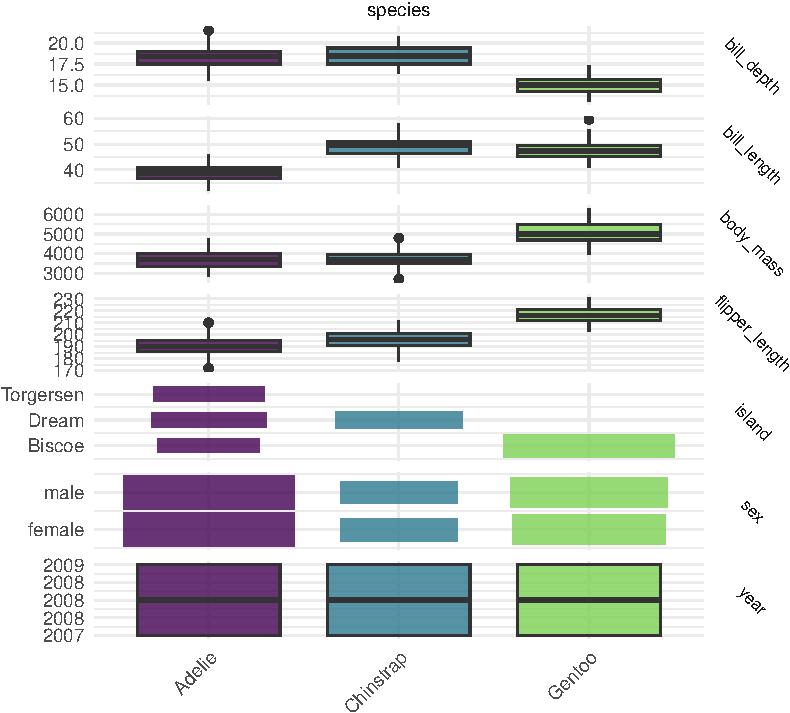
\includegraphics[width=1\textwidth,height=\textheight]{chapters/chapter2/data_and_basic_modeling_files/figure-pdf/fig-penguins-overview-1.pdf}

}

\caption{\label{fig-penguins-overview}Overview of part of the penguins
dataset.}

\end{figure}

\hypertarget{sec-basics-classif-learner}{%
\subsection{LearnerClassif and
MeasureClassif}\label{sec-basics-classif-learner}}

Classification learners, which inherit from
\href{https://mlr3.mlr-org.com/reference/LearnerClassif.html}{\texttt{LearnerClassif}}\index{\texttt{LearnerClassif}}{\marginnote{\begin{footnotesize}\texttt{LearnerClassif}\end{footnotesize}}},
have nearly the same interface as regression learners. However, a key
difference is that the possible predictions in classification are either
\texttt{"response"} -- predicting an observation's class (a penguin's
species in our example, this is sometimes called ``hard labeling'') --
or \texttt{"prob"} -- predicting a vector of probabilities, also called
``posterior probabilities'', of an observation belonging to each class.
In classification, the latter can be more useful as it provides
information about the confidence of the predictions:

\begin{Shaded}
\begin{Highlighting}[]
\NormalTok{lrn\_rpart }\OtherTok{=} \FunctionTok{lrn}\NormalTok{(}\StringTok{"classif.rpart"}\NormalTok{, }\AttributeTok{predict\_type =} \StringTok{"prob"}\NormalTok{)}
\NormalTok{lrn\_rpart}\SpecialCharTok{$}\FunctionTok{train}\NormalTok{(tsk\_penguins, splits}\SpecialCharTok{$}\NormalTok{train)}
\NormalTok{prediction }\OtherTok{=}\NormalTok{ lrn\_rpart}\SpecialCharTok{$}\FunctionTok{predict}\NormalTok{(tsk\_penguins, splits}\SpecialCharTok{$}\NormalTok{test)}
\NormalTok{prediction}
\end{Highlighting}
\end{Shaded}

\begin{verbatim}
<PredictionClassif> for 113 observations:
    row_ids     truth  response prob.Adelie prob.Chinstrap prob.Gentoo
          2    Adelie    Adelie     0.97030         0.0297     0.00000
          4    Adelie    Adelie     0.97030         0.0297     0.00000
          7    Adelie    Adelie     0.97030         0.0297     0.00000
---                                                                   
        338 Chinstrap Chinstrap     0.04651         0.9302     0.02326
        341 Chinstrap    Adelie     0.97030         0.0297     0.00000
        344 Chinstrap Chinstrap     0.04651         0.9302     0.02326
\end{verbatim}

Notice how the predictions include the predicted probabilities for all
three classes, as well as the \texttt{response}, which (by default) is
the class with the highest predicted probability.

Also, the interface for classification measures, which are of class
\href{https://mlr3.mlr-org.com/reference/MeasureClassif.html}{\texttt{MeasureClassif}}\index{\texttt{MeasureClassif}}{\marginnote{\begin{footnotesize}\texttt{MeasureClassif}\end{footnotesize}}},
is identical to regression measures. The key difference in usage is that
you will need to ensure your selected measure evaluates the prediction
type of interest.\index{\texttt{Measure}!\texttt{\$predict\_type}} To
evaluate \texttt{"response"} predictions, you will need measures with
\texttt{predict\_type\ =\ "response"}, or to evaluate probability
predictions you will need \texttt{predict\_type\ =\ "prob"}. The easiest
way to find these measures is by filtering the
\href{https://mlr3.mlr-org.com/reference/mlr_measures.html}{\texttt{mlr\_measures}}
dictionary:

\begin{Shaded}
\begin{Highlighting}[]
\FunctionTok{as.data.table}\NormalTok{(}\FunctionTok{msr}\NormalTok{())[}
\NormalTok{    task\_type }\SpecialCharTok{==} \StringTok{"classif"} \SpecialCharTok{\&}\NormalTok{ predict\_type }\SpecialCharTok{==} \StringTok{"prob"} \SpecialCharTok{\&}
    \SpecialCharTok{!}\FunctionTok{sapply}\NormalTok{(task\_properties, }\ControlFlowTok{function}\NormalTok{(x) }\StringTok{"twoclass"} \SpecialCharTok{\%in\%}\NormalTok{ x)]}
\end{Highlighting}
\end{Shaded}

\begin{verbatim}
                 key                                      label
1:   classif.logloss                                   Log Loss
2: classif.mauc_au1p    Weighted average 1 vs. 1 multiclass AUC
3: classif.mauc_au1u             Average 1 vs. 1 multiclass AUC
4: classif.mauc_aunp Weighted average 1 vs. rest multiclass AUC
5: classif.mauc_aunu          Average 1 vs. rest multiclass AUC
6:    classif.mbrier                     Multiclass Brier Score
4 variables not shown: [task_type, packages, predict_type, task_properties]
\end{verbatim}

We also filtered to remove any measures that have the
\texttt{"twoclass"} property as this would conflict with our
\texttt{"multiclass"} task. We need to use \texttt{sapply} for this, the
\texttt{task\_properties} column is a list column. We can evaluate the
quality of our probability predictions and response predictions
simultaneously by providing multiple measures:

\begin{Shaded}
\begin{Highlighting}[]
\NormalTok{measures }\OtherTok{=} \FunctionTok{msrs}\NormalTok{(}\FunctionTok{c}\NormalTok{(}\StringTok{"classif.mbrier"}\NormalTok{, }\StringTok{"classif.logloss"}\NormalTok{, }\StringTok{"classif.acc"}\NormalTok{))}
\NormalTok{prediction}\SpecialCharTok{$}\FunctionTok{score}\NormalTok{(measures)}
\end{Highlighting}
\end{Shaded}

\begin{verbatim}
 classif.mbrier classif.logloss     classif.acc 
         0.1017          0.2291          0.9469 
\end{verbatim}

The accuracy\index{accuracy} measure evaluates the \texttt{"response"}
predictions whereas the Brier score\index{Brier score}
(\texttt{"classif.mbrier"}, squared difference between predicted
probabilities and the truth) and logloss\index{logloss}
(\texttt{"classif.logloss"}, negative logarithm of the predicted
probability for the true class) are evaluating the probability
predictions.

If no measure is passed to
\texttt{\$score()}\index{\texttt{Prediction}!\texttt{\$score()}}, the
default is the classification error\index{classification error}
(\texttt{msr("classif.ce")}), which is the number of misclassifications
divided by the number of predictions, i.e., \(1 -\)
\texttt{msr("classif.acc")}.

\hypertarget{sec-classif-prediction}{%
\subsection{\texorpdfstring{\texttt{PredictionClassif}, Confusion
Matrix, and
Thresholding}{PredictionClassif, Confusion Matrix, and Thresholding}}\label{sec-classif-prediction}}

\href{https://mlr3.mlr-org.com/reference/PredictionClassif.html}{\texttt{PredictionClassif}}\index{\texttt{PredictionClassif}}{\marginnote{\begin{footnotesize}\texttt{PredictionClassif}\end{footnotesize}}}
objects have two important differences from their regression analog.
Firstly, the added field \texttt{\$confusion}, and secondly the added
method
\texttt{\$set\_threshold()}\index{\texttt{PredictionClassif}!\texttt{\$set\_threshold()}}.

\hypertarget{confusion-matrix}{%
\subsubsection*{Confusion matrix}\label{confusion-matrix}}

A confusion
matrix\index{confusion matrix}{\marginnote{\begin{footnotesize}Confusion
Matrix\end{footnotesize}}} is a popular way to show the quality of
classification (response) predictions in a more detailed fashion by
seeing if a model is good at (mis)classifying observations in a
particular class. For binary and multiclass classification, the
confusion matrix is stored in the
\texttt{\$confusion}\index{\texttt{PredictionClassif}!\texttt{\$confusion}}{\marginnote{\begin{footnotesize}\$confusion\end{footnotesize}}}
field of the
\href{https://mlr3.mlr-org.com/reference/PredictionClassif.html}{\texttt{PredictionClassif}}
object:

\begin{Shaded}
\begin{Highlighting}[]
\NormalTok{prediction}\SpecialCharTok{$}\NormalTok{confusion}
\end{Highlighting}
\end{Shaded}

\begin{verbatim}
           truth
response    Adelie Chinstrap Gentoo
  Adelie        49         3      0
  Chinstrap      1        18      1
  Gentoo         0         1     40
\end{verbatim}

The rows in a confusion matrix are the predicted class and the columns
are the true class. All off-diagonal entries are incorrectly classified
observations, and all diagonal entries are correctly classified. In this
case, the classifier does fairly well classifying all penguins, but we
could have found that it only classifies the Adelie species well but
often conflates Chinstrap and Gentoo, for example.

You can visualize the predicted class labels with
\texttt{autoplot.PredictionClassif()}.

\begin{Shaded}
\begin{Highlighting}[]
\FunctionTok{autoplot}\NormalTok{(prediction)}
\end{Highlighting}
\end{Shaded}

\begin{figure}

{\centering 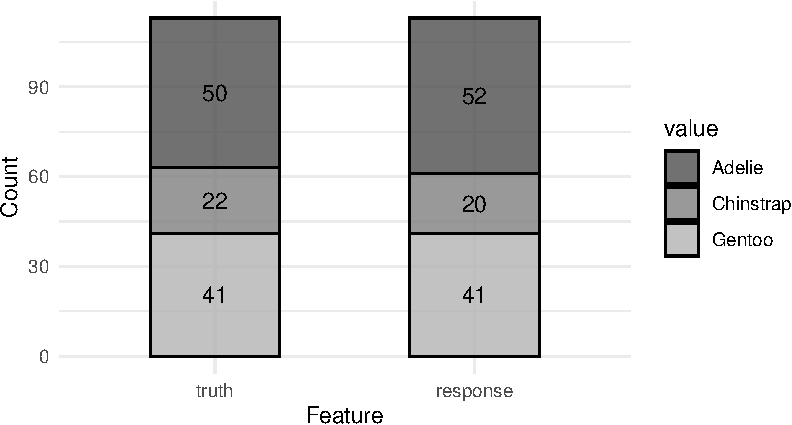
\includegraphics[width=0.7\textwidth,height=\textheight]{chapters/chapter2/data_and_basic_modeling_files/figure-pdf/fig-basics-classlabels-1.pdf}

}

\caption{\label{fig-basics-classlabels}Counts of each class label in the
ground truth data (left) and predictions (right).}

\end{figure}

In the binary classification case, the top left entry corresponds to
true positives\index{true positives}, the top right to false
positives\index{false positives}, the bottom left to false
negatives\index{false negatives} and the bottom right to true
negatives\index{true negatives}. Taking \texttt{tsk\_sonar} as an
example with \texttt{M} as the positive class:

\begin{Shaded}
\begin{Highlighting}[]
\NormalTok{splits }\OtherTok{=} \FunctionTok{partition}\NormalTok{(tsk\_sonar)}
\NormalTok{lrn\_rpart}\SpecialCharTok{$}
  \FunctionTok{train}\NormalTok{(tsk\_sonar, splits}\SpecialCharTok{$}\NormalTok{train)}\SpecialCharTok{$}
  \FunctionTok{predict}\NormalTok{(tsk\_sonar, splits}\SpecialCharTok{$}\NormalTok{test)}\SpecialCharTok{$}
\NormalTok{  confusion}
\end{Highlighting}
\end{Shaded}

\begin{verbatim}
        truth
response  M  R
       M 27 10
       R 10 22
\end{verbatim}

We will return to the concept of binary (mis)classification in greater
detail in Section~\ref{sec-roc}.

\hypertarget{thresholding}{%
\subsubsection*{Thresholding}\label{thresholding}}

The final big difference compared to regression we will discuss is
thresholding\index{thresholding}{\marginnote{\begin{footnotesize}Thresholding\end{footnotesize}}}.
We saw previously that the default \texttt{response} prediction type is
the class with the highest predicted probability. For \texttt{k} classes
with predicted probabilities \(p_1,\dots,p_k\), this is the same as
saying \texttt{response} = argmax\(\{p_1,\dots,p_k\}\). If the maximum
probability is not unique, i.e., multiple classes are predicted to have
the highest probability, then the response is chosen randomly from
these. In binary classification, this means that the positive class will
be selected if the predicted class is greater than 50\%, and the
negative class otherwise.

This 50\% value is known as the threshold and it can be useful to change
this threshold if there is class imbalance (when one class is over- or
under-represented in a dataset), or if there are different costs
associated with classes, or simply if there is a preference to
`over'-predict one class. As an example, let us take
\texttt{tsk("german\_credit")} in which 700 customers have good credit
and 300 have bad. Now we could easily build a model with around ``70\%''
accuracy simply by always predicting a customer will have good credit:

\begin{Shaded}
\begin{Highlighting}[]
\NormalTok{task\_credit }\OtherTok{=} \FunctionTok{tsk}\NormalTok{(}\StringTok{"german\_credit"}\NormalTok{)}
\NormalTok{lrn\_featureless }\OtherTok{=} \FunctionTok{lrn}\NormalTok{(}\StringTok{"classif.featureless"}\NormalTok{, }\AttributeTok{predict\_type =} \StringTok{"prob"}\NormalTok{)}
\NormalTok{split }\OtherTok{=} \FunctionTok{partition}\NormalTok{(task\_credit)}
\NormalTok{lrn\_featureless}\SpecialCharTok{$}\FunctionTok{train}\NormalTok{(task\_credit, split}\SpecialCharTok{$}\NormalTok{train)}
\NormalTok{prediction }\OtherTok{=}\NormalTok{ lrn\_featureless}\SpecialCharTok{$}\FunctionTok{predict}\NormalTok{(task\_credit, split}\SpecialCharTok{$}\NormalTok{test)}
\NormalTok{prediction}\SpecialCharTok{$}\FunctionTok{score}\NormalTok{(}\FunctionTok{msr}\NormalTok{(}\StringTok{"classif.acc"}\NormalTok{))}
\end{Highlighting}
\end{Shaded}

\begin{verbatim}
classif.acc 
        0.7 
\end{verbatim}

\begin{Shaded}
\begin{Highlighting}[]
\FunctionTok{autoplot}\NormalTok{(prediction)}
\end{Highlighting}
\end{Shaded}

\begin{figure}

{\centering 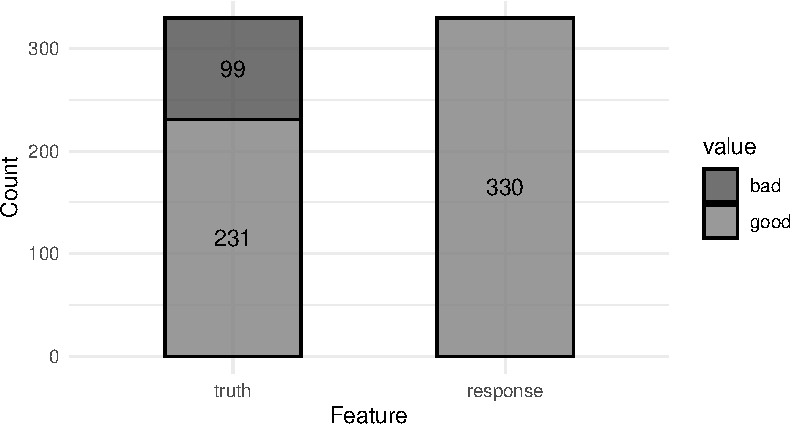
\includegraphics[width=0.7\textwidth,height=\textheight]{chapters/chapter2/data_and_basic_modeling_files/figure-pdf/fig-basics-classlabels-german-1.pdf}

}

\caption{\label{fig-basics-classlabels-german}Class labels ground truth
(left) and predictions (right). The learner completely ignores the `bad'
class.}

\end{figure}

While this model may appear to have good performance on the surface, in
fact, it just ignores all `bad' customers -- this can create big
problems in this finance example, as well as in healthcare tasks and
other settings where false positives\index{false positives} cost more
than false negatives\index{false negatives} (see
Section~\ref{sec-cost-sens} for cost-sensitive classification).

Thresholding allows classes to be selected with a different probability
threshold, so instead of predicting that a customer has bad credit if
P(good) \textless{} 50\%, we might predict bad credit if P(good)
\textless{} 70\% -- notice how we write this in terms of the positive
class, which in this task is `good'. Let us see this in practice:

\begin{Shaded}
\begin{Highlighting}[]
\NormalTok{prediction}\SpecialCharTok{$}\FunctionTok{set\_threshold}\NormalTok{(}\FloatTok{0.7}\NormalTok{)}
\NormalTok{prediction}\SpecialCharTok{$}\FunctionTok{score}\NormalTok{(}\FunctionTok{msr}\NormalTok{(}\StringTok{"classif.acc"}\NormalTok{))}
\end{Highlighting}
\end{Shaded}

\begin{verbatim}
classif.acc 
     0.5394 
\end{verbatim}

\begin{Shaded}
\begin{Highlighting}[]
\NormalTok{lrn\_rpart }\OtherTok{=} \FunctionTok{lrn}\NormalTok{(}\StringTok{"classif.rpart"}\NormalTok{, }\AttributeTok{predict\_type =} \StringTok{"prob"}\NormalTok{)}
\NormalTok{lrn\_rpart}\SpecialCharTok{$}\FunctionTok{train}\NormalTok{(task\_credit, split}\SpecialCharTok{$}\NormalTok{train)}
\NormalTok{prediction }\OtherTok{=}\NormalTok{ lrn\_rpart}\SpecialCharTok{$}\FunctionTok{predict}\NormalTok{(task\_credit, split}\SpecialCharTok{$}\NormalTok{test)}
\NormalTok{prediction}\SpecialCharTok{$}\FunctionTok{score}\NormalTok{(}\FunctionTok{msr}\NormalTok{(}\StringTok{"classif.acc"}\NormalTok{))}
\end{Highlighting}
\end{Shaded}

\begin{verbatim}
classif.acc 
     0.6939 
\end{verbatim}

\begin{Shaded}
\begin{Highlighting}[]
\NormalTok{prediction}\SpecialCharTok{$}\NormalTok{confusion}
\end{Highlighting}
\end{Shaded}

\begin{verbatim}
        truth
response good bad
    good  194  64
    bad    37  35
\end{verbatim}

\begin{Shaded}
\begin{Highlighting}[]
\NormalTok{prediction}\SpecialCharTok{$}\FunctionTok{set\_threshold}\NormalTok{(}\FloatTok{0.7}\NormalTok{)}
\NormalTok{prediction}\SpecialCharTok{$}\FunctionTok{score}\NormalTok{(}\FunctionTok{msr}\NormalTok{(}\StringTok{"classif.acc"}\NormalTok{))}
\end{Highlighting}
\end{Shaded}

\begin{verbatim}
classif.acc 
     0.6879 
\end{verbatim}

\begin{Shaded}
\begin{Highlighting}[]
\NormalTok{prediction}\SpecialCharTok{$}\NormalTok{confusion}
\end{Highlighting}
\end{Shaded}

\begin{verbatim}
        truth
response good bad
    good  181  53
    bad    50  46
\end{verbatim}

While our model performs `worse' overall, i.e.~with lower accuracy, it
is still a `better' model as it more accurately captures the
relationship between classes.

In the binary classification setting, \texttt{\$set\_threshold()} only
requires one numeric argument, which corresponds with the threshold for
the positive class -- hence it is essential to ensure the positive class
is correctly set in your task.

In multiclass classification, thresholding works by first assigning a
threshold to each of the \texttt{n} classes, dividing the predicted
probabilities for each class by these thresholds to return \texttt{n}
ratios, and then the class with the highest ratio is selected. For
example, say we are predicting if a new observation will be of class A,
B, C, or D and we have predicted
\(P(A = 0.2), P(B = 0.4), P(C = 0.1), P(D = 0.3)\). We will assume that
the threshold for all classes is identical and \texttt{1}:

\begin{Shaded}
\begin{Highlighting}[]
\NormalTok{probs }\OtherTok{=} \FunctionTok{c}\NormalTok{(}\FloatTok{0.2}\NormalTok{, }\FloatTok{0.4}\NormalTok{, }\FloatTok{0.1}\NormalTok{, }\FloatTok{0.3}\NormalTok{)}
\NormalTok{thresholds }\OtherTok{=} \FunctionTok{c}\NormalTok{(}\AttributeTok{A =} \DecValTok{1}\NormalTok{, }\AttributeTok{B =} \DecValTok{1}\NormalTok{, }\AttributeTok{C =} \DecValTok{1}\NormalTok{, }\AttributeTok{D =} \DecValTok{1}\NormalTok{)}
\NormalTok{probs}\SpecialCharTok{/}\NormalTok{thresholds}
\end{Highlighting}
\end{Shaded}

\begin{verbatim}
  A   B   C   D 
0.2 0.4 0.1 0.3 
\end{verbatim}

We would therefore predict our observation is of class B as this is the
highest ratio. However, we could change our thresholds so that D has the
lowest threshold and is most likely to be predicted, A has the highest
threshold, and B and C have equal thresholds:

\begin{Shaded}
\begin{Highlighting}[]
\NormalTok{thresholds }\OtherTok{=} \FunctionTok{c}\NormalTok{(}\AttributeTok{A =} \FloatTok{0.5}\NormalTok{, }\AttributeTok{B =} \FloatTok{0.25}\NormalTok{, }\AttributeTok{C =} \FloatTok{0.25}\NormalTok{, }\AttributeTok{D =} \FloatTok{0.1}\NormalTok{)}
\NormalTok{probs}\SpecialCharTok{/}\NormalTok{thresholds}
\end{Highlighting}
\end{Shaded}

\begin{verbatim}
  A   B   C   D 
0.4 1.6 0.4 3.0 
\end{verbatim}

Now our observation will be predicted to be in class D.

In \texttt{mlr3}, this is achieved by passing a named list to
\texttt{\$set\_threshold()}. This is demonstrated below with
\texttt{tsk("zoo")}. Before changing the thresholds, some classes are
never predicted and some are predicted more often than they occur.

\begin{Shaded}
\begin{Highlighting}[]
\FunctionTok{library}\NormalTok{(ggplot2)}
\FunctionTok{library}\NormalTok{(patchwork)}

\NormalTok{tsk\_zoo }\OtherTok{=} \FunctionTok{tsk}\NormalTok{(}\StringTok{"zoo"}\NormalTok{)}
\NormalTok{splits }\OtherTok{=} \FunctionTok{partition}\NormalTok{(tsk\_zoo)}
\NormalTok{lrn\_rpart }\OtherTok{=} \FunctionTok{lrn}\NormalTok{(}\StringTok{"classif.rpart"}\NormalTok{, }\AttributeTok{predict\_type =} \StringTok{"prob"}\NormalTok{)}
\NormalTok{lrn\_rpart}\SpecialCharTok{$}\FunctionTok{train}\NormalTok{(tsk\_zoo, splits}\SpecialCharTok{$}\NormalTok{train)}
\NormalTok{prediction }\OtherTok{=}\NormalTok{ lrn\_rpart}\SpecialCharTok{$}\FunctionTok{predict}\NormalTok{(tsk\_zoo, splits}\SpecialCharTok{$}\NormalTok{test)}
\NormalTok{before }\OtherTok{=} \FunctionTok{autoplot}\NormalTok{(prediction) }\SpecialCharTok{+} \FunctionTok{ggtitle}\NormalTok{(}\StringTok{"Default thresholds"}\NormalTok{)}
\NormalTok{new\_thresh }\OtherTok{=} \FunctionTok{proportions}\NormalTok{(}\FunctionTok{table}\NormalTok{(tsk\_zoo}\SpecialCharTok{$}\FunctionTok{truth}\NormalTok{(splits}\SpecialCharTok{$}\NormalTok{train)))}
\NormalTok{new\_thresh}
\end{Highlighting}
\end{Shaded}

\begin{verbatim}

       mammal          bird       reptile          fish     amphibian 
      0.40299       0.19403       0.04478       0.13433       0.04478 
       insect mollusc.et.al 
      0.07463       0.10448 
\end{verbatim}

\begin{Shaded}
\begin{Highlighting}[]
\NormalTok{prediction}\SpecialCharTok{$}\FunctionTok{set\_threshold}\NormalTok{(new\_thresh)}
\NormalTok{after }\OtherTok{=} \FunctionTok{autoplot}\NormalTok{(prediction) }\SpecialCharTok{+} \FunctionTok{ggtitle}\NormalTok{(}\StringTok{"Inverse weighting thresholds"}\NormalTok{)}
\NormalTok{before }\SpecialCharTok{+}\NormalTok{ after }\SpecialCharTok{+} \FunctionTok{plot\_layout}\NormalTok{(}\AttributeTok{guides =} \StringTok{"collect"}\NormalTok{)}
\end{Highlighting}
\end{Shaded}

\begin{figure}[H]

{\centering 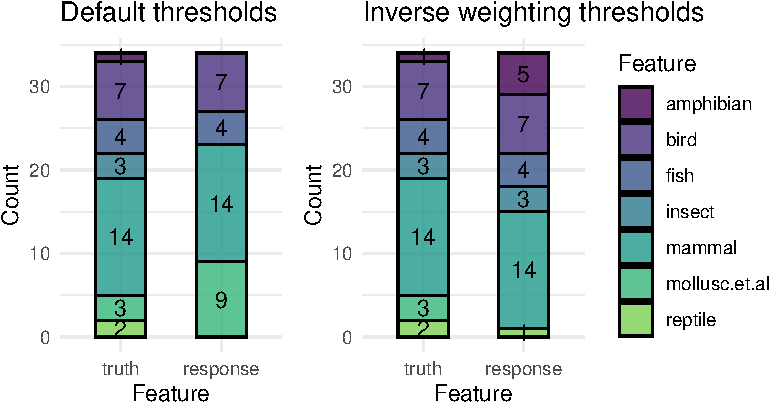
\includegraphics[width=1\textwidth,height=\textheight]{chapters/chapter2/data_and_basic_modeling_files/figure-pdf/fig-zoopreds-1.pdf}

}

\caption{\label{fig-zoopreds}Comparing predicted and ground truth values
for the zoo dataset.}

\end{figure}

Again we see that the model better represents all classes after
thresholding. In this example we set the new thresholds to be the
proportions of each class in the training set. This is known as inverse
weighting\index{inverse weighting}, as we divide the predicted
probability by these class proportions before we select the label with
the highest ratio.

In Section~\ref{sec-cost-sens} we will look at cost-sensitive
classification\index{classification!cost-sensitive} where each cell in
the confusion matrix has a different associated cost.

\hypertarget{sec-row-col-roles}{%
\section{Task Column Roles}\label{sec-row-col-roles}}

\begin{tcolorbox}[enhanced jigsaw, colframe=quarto-callout-note-color-frame, rightrule=.15mm, bottomrule=.15mm, toprule=.15mm, opacityback=0, colback=white, left=2mm, arc=.35mm, breakable, leftrule=.75mm]
\begin{minipage}[t]{5.5mm}
\textcolor{quarto-callout-note-color}{\faInfo}
\end{minipage}%
\begin{minipage}[t]{\textwidth - 5.5mm}

\textbf{This section covers advanced ML or technical
details.}\vspace{2mm}

\end{minipage}%
\end{tcolorbox}

Now that we have covered regression and classification, we will briefly
return to tasks and in particular to column roles\index{column roles},
which are used to customize tasks further. Column roles are used by
\texttt{Task} objects to define important metadata that can be used by
learners and other objects to interact with the task. True to their
name, they assign particular roles to columns in the data, we have
already seen some of these in action with targets and features. There
are seven column roles:

\begin{enumerate}
\def\labelenumi{\arabic{enumi}.}
\tightlist
\item
  \texttt{"feature"}: Features used for prediction.
\item
  \texttt{"target"}: Target variable to predict.
\item
  \texttt{"name"}: Row names/observation labels, e.g., for
  \texttt{mtcars} this is the \texttt{"model"} column.
\item
  \texttt{"order"}: Variable(s) used to order data returned by
  \texttt{\$data()}; must be sortable with \texttt{order()}.
\item
  \texttt{"group"}: Variable used to keep observations together during
  resampling.
\item
  \texttt{"stratum"}: Variable(s) to stratify during resampling.
\item
  \texttt{"weight"}: Observation weights. Only one numeric column may
  have this role.
\end{enumerate}

We have already seen how features and targets work in
Section~\ref{sec-tasks}, which are the only column roles that each task
must have. In Section~\ref{sec-strat-group} we will have a look at the
\texttt{stratum} and \texttt{group} column roles. So, for now, we will
only look at \texttt{order}, and \texttt{weight}. We will not go into
detail about \texttt{name}, which is primarily used in plotting and will
almost always be the \texttt{rownames()} of the underlying data.

Column roles are updated using
\texttt{\$set\_col\_roles()}\index{\texttt{Task}!\texttt{\$set\_col\_roles()}}.
When we set the \texttt{"order"} column role, the data is ordered
according to that column(s). In the following example, we set the
\texttt{"order"} column role and then order data by this column by
including \texttt{ordered\ =\ TRUE}:

\begin{Shaded}
\begin{Highlighting}[]
\NormalTok{df }\OtherTok{=} \FunctionTok{data.frame}\NormalTok{(mtcars[}\DecValTok{1}\SpecialCharTok{:}\DecValTok{2}\NormalTok{, ], }\AttributeTok{idx =} \DecValTok{2}\SpecialCharTok{:}\DecValTok{1}\NormalTok{)}
\NormalTok{tsk\_mtcars\_order }\OtherTok{=} \FunctionTok{as\_task\_regr}\NormalTok{(df, }\AttributeTok{target =} \StringTok{"mpg"}\NormalTok{)}
\CommentTok{\# original order}
\NormalTok{tsk\_mtcars\_order}\SpecialCharTok{$}\FunctionTok{data}\NormalTok{(}\AttributeTok{ordered =} \ConstantTok{TRUE}\NormalTok{)}
\end{Highlighting}
\end{Shaded}

\begin{verbatim}
   mpg am carb cyl disp drat gear  hp idx  qsec vs    wt
1:  21  1    4   6  160  3.9    4 110   2 16.46  0 2.620
2:  21  1    4   6  160  3.9    4 110   1 17.02  0 2.875
\end{verbatim}

\begin{Shaded}
\begin{Highlighting}[]
\CommentTok{\# order by "idx" column}
\NormalTok{tsk\_mtcars\_order}\SpecialCharTok{$}\FunctionTok{set\_col\_roles}\NormalTok{(}\StringTok{"idx"}\NormalTok{, }\AttributeTok{roles =} \StringTok{"order"}\NormalTok{)}
\NormalTok{tsk\_mtcars\_order}\SpecialCharTok{$}\FunctionTok{data}\NormalTok{(}\AttributeTok{ordered =} \ConstantTok{TRUE}\NormalTok{)}
\end{Highlighting}
\end{Shaded}

\begin{verbatim}
   mpg am carb cyl disp drat gear  hp  qsec vs    wt
1:  21  1    4   6  160  3.9    4 110 17.02  0 2.875
2:  21  1    4   6  160  3.9    4 110 16.46  0 2.620
\end{verbatim}

In this example we can see that by setting \texttt{"idx"} to have the
\texttt{"order"} column role, it is no longer used as a feature when we
run \texttt{\$data()} but instead is used to order the observations
according to its value. This metadata is not passed to a learner.

The \texttt{weights} column role is used to weight data points
differently. One example of why we would do this is in classification
tasks with severe class imbalance, where weighting the minority class
more heavily may improve the model's predictive performance for that
class. For example in the \texttt{breast\_cancer} dataset, there are
more instances of benign tumors than malignant tumors, so if we want to
better predict malignant tumors we could weight the data in favor of
this class:

\begin{Shaded}
\begin{Highlighting}[]
\NormalTok{cancer\_unweighted }\OtherTok{=} \FunctionTok{tsk}\NormalTok{(}\StringTok{"breast\_cancer"}\NormalTok{)}
\FunctionTok{summary}\NormalTok{(cancer\_unweighted}\SpecialCharTok{$}\FunctionTok{data}\NormalTok{()}\SpecialCharTok{$}\NormalTok{class)}
\end{Highlighting}
\end{Shaded}

\begin{verbatim}
malignant    benign 
      239       444 
\end{verbatim}

\begin{Shaded}
\begin{Highlighting}[]
\CommentTok{\# add column where weight is 2 if class "malignant", and 1 otherwise}
\NormalTok{df }\OtherTok{=}\NormalTok{ cancer\_unweighted}\SpecialCharTok{$}\FunctionTok{data}\NormalTok{()}
\NormalTok{df}\SpecialCharTok{$}\NormalTok{weights }\OtherTok{=} \FunctionTok{ifelse}\NormalTok{(df}\SpecialCharTok{$}\NormalTok{class }\SpecialCharTok{==} \StringTok{"malignant"}\NormalTok{, }\DecValTok{2}\NormalTok{, }\DecValTok{1}\NormalTok{)}

\CommentTok{\# create new task and role}
\NormalTok{cancer\_weighted }\OtherTok{=} \FunctionTok{as\_task\_classif}\NormalTok{(df, }\AttributeTok{target =} \StringTok{"class"}\NormalTok{)}
\NormalTok{cancer\_weighted}\SpecialCharTok{$}\FunctionTok{set\_col\_roles}\NormalTok{(}\StringTok{"weights"}\NormalTok{, }\AttributeTok{roles =} \StringTok{"weight"}\NormalTok{)}

\CommentTok{\# compare weighted and unweighted predictions}
\NormalTok{split }\OtherTok{=} \FunctionTok{partition}\NormalTok{(cancer\_unweighted)}
\NormalTok{lrn\_rf }\OtherTok{=} \FunctionTok{lrn}\NormalTok{(}\StringTok{"classif.ranger"}\NormalTok{)}
\NormalTok{lrn\_rf}\SpecialCharTok{$}\FunctionTok{train}\NormalTok{(cancer\_unweighted, split}\SpecialCharTok{$}\NormalTok{train)}\SpecialCharTok{$}
  \FunctionTok{predict}\NormalTok{(cancer\_unweighted, split}\SpecialCharTok{$}\NormalTok{test)}\SpecialCharTok{$}\FunctionTok{score}\NormalTok{()}
\end{Highlighting}
\end{Shaded}

\begin{verbatim}
classif.ce 
    0.0177 
\end{verbatim}

\begin{Shaded}
\begin{Highlighting}[]
\NormalTok{lrn\_rf}\SpecialCharTok{$}\FunctionTok{train}\NormalTok{(cancer\_weighted, split}\SpecialCharTok{$}\NormalTok{train)}\SpecialCharTok{$}
  \FunctionTok{predict}\NormalTok{(cancer\_weighted, split}\SpecialCharTok{$}\NormalTok{test)}\SpecialCharTok{$}\FunctionTok{score}\NormalTok{()}
\end{Highlighting}
\end{Shaded}

\begin{verbatim}
classif.ce 
   0.00885 
\end{verbatim}

In this example, weighting improves the overall model performance (but
see Chapter~\ref{sec-performance} for more thorough comparison methods).
Not all models can handle weights in tasks so check a learner's
properties to make sure this column role is being used as expected.

\hypertarget{sec-lrns-add}{%
\section{Supported Learning Algorithms}\label{sec-lrns-add}}

\texttt{mlr3} supports many learning algorithms (some with multiple
implementations) as \texttt{Learner}s. These are primarily provided by
the \href{https://mlr3.mlr-org.com}{\texttt{mlr3}}\index{\texttt{mlr3}},
\href{https://mlr3learners.mlr-org.com}{\texttt{mlr3learners}}\index{\texttt{mlr3learners}}
and
\href{https://mlr3extralearners.mlr-org.com}{\texttt{mlr3extralearners}}\index{\texttt{mlr3extralearners}}
packages. However, all packages that implement new tasks
(Chapter~\ref{sec-special}) also include a handful of simple algorithms.

The list of learners included in \texttt{mlr3} is deliberately small to
avoid large sets of dependencies:

\begin{itemize}
\tightlist
\item
  Featureless learners
  (\texttt{"regr.featureless"}/\texttt{"classif.featureless"}), which
  are baseline learners (Section~\ref{sec-basics-featureless}).
\item
  Debug learners (\texttt{"regr.debug"}/\texttt{"classif.debug"}), which
  are used to debug code (Section~\ref{sec-error-handling}).
\item
  Classification and regression trees (also known as CART:
  \texttt{"regr.rpart"}/\texttt{"classif.rpart"}).
\end{itemize}

The
\href{https://mlr3learners.mlr-org.com}{\texttt{mlr3learners}}\index{\texttt{mlr3learners}}
package contains a selection of algorithms (and select implementations)
chosen by the mlr team that we recommend as a good starting point for
most experiments:

\begin{itemize}
\tightlist
\item
  Linear (\texttt{"regr.lm"}) and logistic (\texttt{"classif.log\_reg"})
  regression\index{logistic regression}.
\item
  Penalized generalized linear models, where the penalization is either
  exposed as a hyperparameter
  (\texttt{"regr.glmnet"}/\texttt{"classif.glmnet"})\index{generalized linear model}
  or where it is optimized automatically
  (\texttt{"regr.cv\_glmnet"}/\texttt{"classif.cv\_glmnet"}).
\item
  Weighted \(k\)-Nearest Neighbors\index{k-nearest neighbors}
  (\texttt{"regr.kknn"}/\texttt{"classif.kknn"}).
\item
  Kriging / Gaussian process\index{Gaussian process} regression
  (\texttt{"regr.km"}).
\item
  Linear (\texttt{"classif.lda"}) and quadratic (\texttt{"classif.qda"})
  discriminant analysis.
\item
  Naïve Bayes classification (\texttt{"classif.naive\_bayes"}).
\item
  Support-vector machines\index{support vector machine}
  (\texttt{"regr.svm"}/\texttt{"classif.svm"}).
\item
  Gradient boosting\index{boosting}
  (\texttt{"regr.xgboost"}/\texttt{"classif.xgboost"}).
\item
  Random forests\index{random forest} for regression and classification
  (\texttt{"regr.ranger"}/\texttt{"classif.ranger"}).
\end{itemize}

The majority of other supported learners are in
\href{https://mlr3extralearners.mlr-org.com}{\texttt{mlr3extralearners}}\index{\texttt{mlr3extralearners}}.
You can find an up-to-date list of learners at
\url{https://mlr-org.com/learners.html}.

The dictionary
\href{https://mlr3.mlr-org.com/reference/mlr_learners.html}{\texttt{mlr\_learners}}\index{\texttt{mlr\_learners}}
contains learners that are supported in loaded packages:

\begin{Shaded}
\begin{Highlighting}[]
\NormalTok{learners\_dt }\OtherTok{=} \FunctionTok{as.data.table}\NormalTok{(mlr\_learners)}
\NormalTok{learners\_dt}
\end{Highlighting}
\end{Shaded}

\begin{verbatim}
                     key                       label task_type
  1:  classif.AdaBoostM1           Adaptive Boosting   classif
  2:         classif.C50            Tree-based Model   classif
  3:         classif.IBk           Nearest Neighbour   classif
  4:         classif.J48            Tree-based Model   classif
  5:        classif.JRip Propositional Rule Learner.   classif
 ---                                                          
134: surv.priority_lasso              Priority Lasso      surv
135:         surv.ranger               Random Forest      surv
136:          surv.rfsrc               Random Forest      surv
137:            surv.svm      Support Vector Machine      surv
138:        surv.xgboost           Gradient Boosting      surv
4 variables not shown: [feature_types, packages, properties, predict_types]
\end{verbatim}

The resulting \texttt{data.table} contains a lot of metadata that is
useful for identifying learners with particular properties. For example,
we can list all learners that support classification problems:

\begin{Shaded}
\begin{Highlighting}[]
\NormalTok{learners\_dt[task\_type }\SpecialCharTok{==} \StringTok{"classif"}\NormalTok{]}
\end{Highlighting}
\end{Shaded}

\begin{verbatim}
                   key                       label task_type
 1: classif.AdaBoostM1           Adaptive Boosting   classif
 2:        classif.C50            Tree-based Model   classif
 3:        classif.IBk           Nearest Neighbour   classif
 4:        classif.J48            Tree-based Model   classif
 5:       classif.JRip Propositional Rule Learner.   classif
---                                                         
40:     classif.ranger                        <NA>   classif
41:      classif.rfsrc               Random Forest   classif
42:      classif.rpart         Classification Tree   classif
43:        classif.svm                        <NA>   classif
44:    classif.xgboost                        <NA>   classif
4 variables not shown: [feature_types, packages, properties, predict_types]
\end{verbatim}

We can filter by multiple conditions, for example to list all regression
learners that can predict standard errors:

\begin{Shaded}
\begin{Highlighting}[]
\NormalTok{learners\_dt[task\_type }\SpecialCharTok{==} \StringTok{"regr"} \SpecialCharTok{\&}
  \FunctionTok{sapply}\NormalTok{(predict\_types, }\ControlFlowTok{function}\NormalTok{(x) }\StringTok{"se"} \SpecialCharTok{\%in\%}\NormalTok{ x)]}
\end{Highlighting}
\end{Shaded}

\begin{verbatim}
                key                                    label task_type
1:       regr.debug             Debug Learner for Regression      regr
2:       regr.earth Multivariate Adaptive Regression Splines      regr
3: regr.featureless           Featureless Regression Learner      regr
4:         regr.gam    Generalized Additive Regression Model      regr
5:         regr.glm            Generalized Linear Regression      regr
6:          regr.km                                     <NA>      regr
7:          regr.lm                                     <NA>      regr
8:         regr.mob       Model-based Recursive Partitioning      regr
9:      regr.ranger                                     <NA>      regr
4 variables not shown: [feature_types, packages, properties, predict_types]
\end{verbatim}

\hypertarget{conclusion}{%
\section{Conclusion}\label{conclusion}}

In this chapter, we covered the building blocks of
\href{https://mlr3.mlr-org.com}{\texttt{mlr3}}\index{\texttt{mlr3}}. We
first introduced basic ML methodology and then showed how this is
implemented in \texttt{mlr3}. We began by looking at the
\href{https://mlr3.mlr-org.com/reference/Task.html}{\texttt{Task}}
class, which is used to define machine learning tasks or problems to
solve. We then looked at the
\href{https://mlr3.mlr-org.com/reference/Learner.html}{\texttt{Learner}}
class, which encapsulates machine learning algorithms, hyperparameters,
and other meta-information. Finally, we considered how to evaluate
machine learning models with objects from the
\href{https://mlr3.mlr-org.com/reference/Measure.html}{\texttt{Measure}}
class. After looking at regression implementations, we extended all the
above to the classification setting, before finally looking at some
extra details about tasks and the learning algorithms that are
implemented across \texttt{mlr3}. The rest of this book will build on
the basic elements seen in this chapter, starting with more advanced
model comparison methods in Chapter~\ref{sec-performance} before moving
on to improve model performance with automated hyperparameter tuning in
Chapter~\ref{sec-optimization}.

\hypertarget{tbl-basics-api}{}
\begin{longtable}[]{@{}
  >{\raggedright\arraybackslash}p{(\columnwidth - 4\tabcolsep) * \real{0.2143}}
  >{\raggedright\arraybackslash}p{(\columnwidth - 4\tabcolsep) * \real{0.3571}}
  >{\raggedright\arraybackslash}p{(\columnwidth - 4\tabcolsep) * \real{0.4286}}@{}}
\caption{\label{tbl-basics-api}Important classes and functions covered
in this chapter with underlying class (if applicable), class constructor
or function, and important class fields and methods (if
applicable).}\tabularnewline
\toprule\noalign{}
\begin{minipage}[b]{\linewidth}\raggedright
Class
\end{minipage} & \begin{minipage}[b]{\linewidth}\raggedright
Constructor/Function
\end{minipage} & \begin{minipage}[b]{\linewidth}\raggedright
Fields/Methods
\end{minipage} \\
\midrule\noalign{}
\endfirsthead
\toprule\noalign{}
\begin{minipage}[b]{\linewidth}\raggedright
Class
\end{minipage} & \begin{minipage}[b]{\linewidth}\raggedright
Constructor/Function
\end{minipage} & \begin{minipage}[b]{\linewidth}\raggedright
Fields/Methods
\end{minipage} \\
\midrule\noalign{}
\endhead
\bottomrule\noalign{}
\endlastfoot
\href{https://mlr3.mlr-org.com/reference/Task.html}{\texttt{Task}} &
\href{https://mlr3.mlr-org.com/reference/mlr_sugar.html}{\texttt{tsk()}}/\href{https://mlr3.mlr-org.com/reference/mlr_sugar.html}{\texttt{tsks()}}/\texttt{as\_task\_X}
& \texttt{\$filter()}; \texttt{\$select()}; \texttt{\$data()} \\
\href{https://mlr3.mlr-org.com/reference/Learner.html}{\texttt{Learner}}
&
\href{https://mlr3.mlr-org.com/reference/mlr_sugar.html}{\texttt{lrn()}}/\href{https://mlr3.mlr-org.com/reference/mlr_sugar.html}{\texttt{lrns()}}
& \texttt{\$train()}; \texttt{\$predict()};
\texttt{\$predict\_newdata()}; \texttt{\$model()} \\
\href{https://mlr3.mlr-org.com/reference/Prediction.html}{\texttt{Prediction}}
& \texttt{some\_learner\$predict()} & \texttt{\$score()};
\texttt{\$set\_threshold()}; \texttt{\$confusion} \\
\href{https://mlr3.mlr-org.com/reference/Measure.html}{\texttt{Measure}}
&
\href{https://mlr3.mlr-org.com/reference/mlr_sugar.html}{\texttt{msr()}}/\href{https://mlr3.mlr-org.com/reference/mlr_sugar.html}{\texttt{msrs()}}
& - \\
\end{longtable}

\hypertarget{exercises}{%
\section{Exercises}\label{exercises}}

\begin{enumerate}
\def\labelenumi{\arabic{enumi}.}
\tightlist
\item
  Train a classification model with the \texttt{classif.rpart} learner
  on the ``Pima Indians Diabetes'' dataset. Do this without using
  \texttt{tsk("pima")}, and instead by constructing a task from the
  dataset in the \texttt{mlbench}-package:
  \texttt{data(PimaIndiansDiabetes2,\ package\ =\ "mlbench")}. Make sure
  to define the \texttt{pos} outcome as positive class. Train the model
  on a random 80\% subset of the given data and evaluate its performance
  with the classification error measure on the remaining data. (Note
  that the data set has NAs in its features. You can either rely on
  \texttt{rpart}`s capability to handle them internally ('surrogate
  splits') or remove them from the initial \texttt{data.frame} by using
  \texttt{na.omit}.
\item
  Calculate the true positive, false positive, true negative, and false
  negative rates of the predictions made by the model in Exercise 1. Try
  to solve this in two ways: (a) Using \texttt{mlr3measures}-predefined
  measure objects, and (b) without using \texttt{mlr3} tools by directly
  working on the ground truth and prediction vectors. Compare the
  results.
\item
  Change the threshold of the model from Exercise 1 such that the false
  positive rate is lower than the false negative rate. What is one
  reason you might do this in practice?
\end{enumerate}
